\documentclass[12pt]{article}
\usepackage[utf8]{inputenc}
\usepackage[T2A,T1]{fontenc}
\usepackage{amssymb}
\usepackage{amsmath}

\usepackage[english,russian]{babel}
\usepackage{csquotes}
\usepackage[backend=biber, style=ieee]{biblatex}

\textwidth 14cm
\textheight 21cm

\usepackage{graphicx}
\graphicspath{ {./images/} }

\addbibresource{article_ru.bib}

\title{Несчётность множества континуум, ещё шах}
\author{Роман Олегович Коротков}

\begin{document}

\selectlanguage{russian}

\begin{flushleft}
{\bf УДК 510.223 }\\{\bf MSC 03E99 }
\end{flushleft}

{\let\newpage\relax\maketitle}

\begin{abstract}

Статья продолжает серию исследований, посвящённых критическому анализу доказательств несчётности континуума. В работе внимание сконцентрировано на геометрических построениях Кантора и переходе от них к его теории порядковых типов. Рассматривается, как Кантор разделил области рефлексивности бесконечности: полиномиальную (где сохраняется подобие части целому) и экспоненциальную (где рефлексивность ограничивается и достигается предикативность). Показывается, что именно это разделение делает геометрические доказательства и диагональный аргумент корректными лишь при соответствующих предположениях о морфологии бесконечности. Анализируется связь аксиом непрерывности, Архимеда и регулярности с ограничением импредикативности. Предлагается интерпретация, согласно которой современная теория множеств существенно упрощает исходную канторовскую картину, отождествляя континуум с множеством степени счётного множества. Рассматриваются альтернативные конструкции (сюрреальные числа, поля большей мощности, модели в логике первого порядка), в которых непрерывность и всюду плотность не влекут автоматической несчётности в сильном смысле. Статья демонстрирует, что конфликт предикативности и импредикативности является структурным свойством упорядочения, а не внутренним свойством самого множества точек.

{\it Ключевые слова: несчётность множества вещественных чисел; порядковые типы Кантора; полиномиальная и экспоненциальная рефлексивность; предикативность и импредикативность; аксиома непрерывности; архимедовость; сюрреальные числа; континуум; поля большоймощности; актуальная и потенциальная бесконечность.}

\end{abstract}

\selectlanguage{english}

\begin{abstract}

The article continues the series of studies devoted to a critical analysis of the proofs of the uncountability of the continuum. The work focuses on Cantor’s geometric constructions and the transition from them to his theory of order types. It examines how Cantor divided the domains of reflexivity of infinity: the polynomial domain (where the similarity of the part to the whole is preserved) and the exponential domain (where reflexivity is restricted and predicativity is achieved). It is shown that precisely this division renders the geometric proofs and the diagonal argument correct only under the corresponding assumptions about the morphology of infinity. The connection between the axioms of continuity, Archimedes and regularity and the restriction of impredicativity is analysed. An interpretation is proposed according to which modern set theory substantially simplifies Cantor’s original picture by identifying the continuum with the power set of a countable set. Alternative constructions are considered (surreal numbers, fields of greater cardinality, models in first-order logic) in which continuity and density do not entail automatic uncountability in the strong sense. The article demonstrates that the conflict between predicativity and impredicativity is a structural property of the ordering rather than an intrinsic property of the set of points itself.

{\it Keywords: uncountability of the reals; Cantor’s order types; polynomial and exponential reflexivity; predicativity and impredicativity; axiom of continuity; Archimedeanness; surreal numbers; continuum; fields of greater cardinality; actual and potential infinity.}

\end{abstract}

\selectlanguage{russian}

Георг Кантор подарил миру одну из самых противоречивых математических теорий, позволившую описывать бесконечность, результаты которой распространились по всем областям человеческих знаний от философии до физики, оказав на них существенное влияние. Однако, судя по всему, идея бесконечного оказалась сложнее и непостижимее, чем можно было бы подумать, и математические методы работы с бесконечными объектами, которые он использовал в своих доказательствах, нуждаются в существенных уточнениях. За многими математическими концепциями стоят бесконечные процедуры, изученность таких процедур и их взаимодействий во времена Кантора, да, пожалуй, и сейчас, не достаточна и требует дополнительных неявных предположений, что становится причиной их слишком вольного применения. Натуральные числа связаны с процедурой счета, непрерывность числовой прямой связана с процедурами построения вещественных чисел, а процедура выбора элементов последовательности обуславливает свойства новой последовательности. Неосторожное сочетание бесконечных математических процедур, например, в диагональном методе, может приводить к серьёзным противоречиям, источники которых сложно обнаружить и исправить.

В статье ''Несчётность множества континуум, шах'' были разобраны границы применимости доказательства несчётности множества действительных чисел диагональным методом Кантора, на основе анализа взаимодействия трёх бесконечных процедур: нумерации, записи вещественного числа и построения отличного от всех элемента. Проблема заключается в том, что определяя зависимые математические процедуры, мы не можем наделить их свойствами, которых лишены те процедуры от которых они зависят, чтобы избежать появления подобных свойств необходимо убедиться в корректности и существовании определяемых процедур, и предположениях которые для этого требуются. Хотя процедурная формулировка более понятна и естественная данный вывод общезначим и легко переформулируется в термины статичной теории: предположения о морфологии бесконечных объектов распространяются и на производные объекты, в частности, на функциональные отношения, которые наследуют такую предполагаемую морфологию. Диагональный метод Кантора, абсолютно корректен если понимать его как доказательство того факта, что множество натуральных чисел не может взаимно однозначно отображаться на множество вещественных чисел, в контексте предположения незамкнутости количественной арифметики. То есть в предположении существования различных форм бесконечного, обладающих свойствами универсальности (воспроизводимости, обеспечивающей одновременное сопоставление элементов бесконечного числа множеств) и тотальности (способности теории распространять конструктивные свойства на все элементы множества). Однако, в отсутствии таких сильных предположений, даже актуальная бесконечность приобретает аморфные черты потенциальной бесконечности. В таком случае, отношение эквивалентности, называемое мощностью, определяет класс эквивалентности неограниченно продолжаемых множеств, которые можно бесконечно поэлементно сопоставлять друг другу. Что приводит к некорректности классического вывода из диагонального построения, равенство мощностей без дополнительных структурных ограничений не означает тождественности в смысле биективного отображения, поскольку само взаимно однозначное соответствие является классом эквивалентности, препятствуя однозначному определению класса эквивалентности диагонального элемента. 

Интерпретацию взаимно однозначного соответствия через биективное отображение мы называем {\it сильной}, а интерпретацию класса эквивалентности неограниченного поэлементного сопоставления не подразумевающего биекцию - {\it слабой}. Современных аксиоматические теории множеств интегрируют сильную интерпретацию ассоциируя её со свойствами универсальности и тотальности, в то время как Кантор, судя по всему, использовал слабую интерпретацию, более аккуратно обозначая границы применимости своих доказательств. Он выстраивает две независимых алгебры с различными морфологиями бесконечности (распространяющимися, в частности, на функциональные отношения): кардинальную и порядковую, однако современные теории не разделяет виды функциональных отношений, сигнализируя о неоднозначности претензий этих теорий на изоморфизм с построениями Кантора. Математическая обоснованность этих претензий является предметом исследования нестоящей серии статей. Кроме того, мы возвращаем в математику понятия актуальной и потенциальной бесконечности, поскольку их переплетение оказывает непосредственное влияние на неоднозначности возникающие в связанных математических процедурах. Для корректности диагонального метода требуется не просто актуальная бесконечность, а актуальная бесконечность обладающая свойством подобия своей части (рефлексивностью) и одновременно довольно жесткой структурой, позволяющей ограничить классы эквивалентности бесконечных множеств. Считается, что современные теории множеств, постулируя актуальную бесконечность, не нуждаются более в концепции потенциальной бесконечности, играющими центральную роль в картине Кантора, что имеет прямое отношение к предмету исследования.

Исторически диагональный аргумент был не первым придуманным Кантором способом доказать, что множество точек на числовой прямой несопоставимо с множеством натуральных чисел. В своей работе 1874 году Кантор применяет бесконечную процедуру построения вложенных интервалов в тесной связи с бесконечной процедурой нумерации вещественных чисел \cite{interval} для доказательства их несчётности на отрезке, а в 1879 дорабатывает это доказательство, используя понятие всюду плотного множества \cite{interval-density}. Впоследствии на основе этих доказательств, было предложено ещё одно доказательство, основанное на лемме о вложенных отрезках, которое можно найти в современных книгах по аналитической математике и теории множеств \cite{matan-interval}, к сожалению нам не удалось проследить его авторство. Стоит отметить, что геометрические доказательства весьма изящны, если не сказать гениальны, запутанные с различием между потенциальной и актуальной бесконечностями, они не позволяли строго обозначить интуитивное ощущение неоднозначности в вопросе выхода за границы их применимости, в течении полутора веков, надёжно защищая диагональный метод и другие вызывающие сомнения в своей универсальности доказательства от критики. Рассмотрим подробнее наиболее часто используемое в настоящее время доказательство.

Теорема: {\sl Множество вещественных чисел отрезка [0, 1] несчётно.}

Доказательство:

Предположим, что точки отрезка [0, 1] можно занумеровать, то есть $[0, 1] = \{x_1, x_2, x_3, \ldots, x_n, \dots\}$. Выберем какой-либо отрезок $[a_1, b_1]$, лежащий на $[0, 1]$ и не содержащий точки $x_1$. Далее выберем отрезок $[a_2, b_2]$, лежащий на $[a_1, b_1]$ и не содержащий точки $x_2$ и так далее (рис. \ref{fig:interval}).

\begin{figure}[htbp]
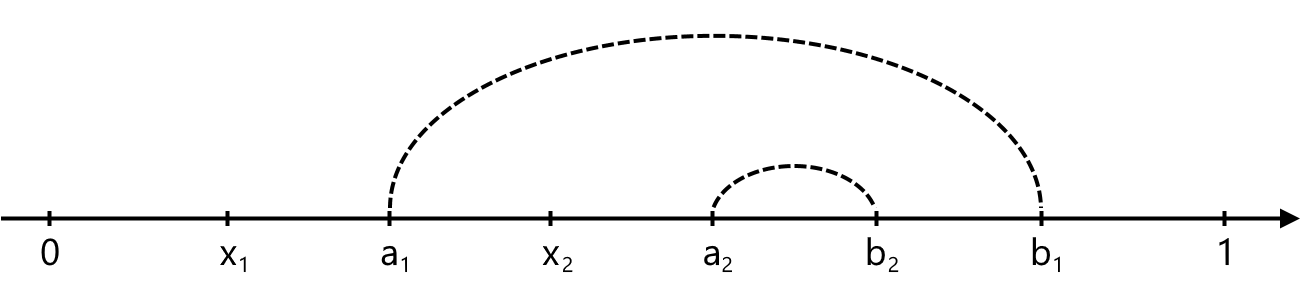
\includegraphics[width=0.80\textwidth, draft=false]{interval}
\centering
\caption{последовательность вложенных отрезков}
\label{fig:interval}
\end{figure}

На шаге $n$ выберем отрезок $[a_n, b_n]$, лежащий на $[a_{n - 1}, b_{n - 1}]$ и не содержащий точки $x_n$:
\begin{align}
\begin{split}
x_1 &\notin [a_1, b_1] \subset [0, 1]\\
x_2 &\notin [a_2, b_2] \subset [0, 1]\\
x_3 &\notin [a_3, b_3] \subset [0, 1]\\
&\ldots\\
x_n &\notin [a_n, b_n] \subset [0, 1]\\
&\ldots 
\label{equ:nested-intervals}
\end{split}
\end{align}

Таким образом, получаем систему вложенных отрезков $[a_n, b_n]$ такую, что ни одна точка $x_n$ не принадлежит пересечению $\bigcap\limits^{\infty}_{n = 1} [a_n, b_n]$, но согласно принципу вложенных отрезков \cite{matan-nested-interval} существует точка, обозначим ее $\xi$, которая принадлежит всем отрезкам $[a_n, b_n]$:
\begin{equation}
\xi \in [a_n, b_n], n = 1, 2, 3, \ldots \label{equ:xi-in-interval}
\end{equation}

Поскольку $[a_n, b_n] \subset [0, 1]$ при всех $n = 1, 2, 3, \ldots$, то $\xi \in [0, 1]$. А так как все точки отрезка [0, 1] по предположению пронумерованы, то точка $\xi$ также должна иметь какой-то номер, то есть существует такое натуральное число $n_0$, что $\xi = x_{n_0}$, и тогда согласно (\ref{equ:xi-in-interval}) получим:
\begin{equation}
x_{n_0} \in [a_n, b_n], n = 1, 2, 3, \ldots 
\end{equation}

В частности $x_{n_0} \in [a_{n_0}, b_{n_0}]$, a это противоречит условию (\ref{equ:nested-intervals}). Следовательно наше предположение не верно.

Как и в статье ''Несчётность множества континуум, шах'' мы откажемся на время от формализма современной теории множеств и рассмотрим доказательства в исторической перспективе, а также в контексте использования без явной отсылки к предположениям и интерпретациям теории множеств. При этом мы будем для сравнения мы будем стараться сопровождать наши размышления комментариями, выражающими современный взгляд на обсуждаемые вопросы. В предыдущей статье были построены два подмножества вещественных чисел $C[0, 1]$ и $U[0, 1]$ в двоичной записи. Напомним, что $U[0, 1]$ можно построить 2 способами: выбирая из отрезка $[0, 1]$ вещественные числа содержащие $1$ в определённом разряде, постоянно увеличивая этот разряд от $1$ до бесконечности, или итеративно добавляя на каждом шаге слагаемое $2^{-i}$ ко всем бесконечным рядам уже содержащимся во множестве, начиная с ряда, все коэффициенты которого равны $0$. $C[0, 1]$ в свою очередь является просто зеркальным отражением натуральных чисел в двоичной записи, либо, повторением процедур построения $U[0, 1]$ ничем не ограниченное (но не бесконечное) количество раз. Для построения мы приняли довольно общую аксиому возможности бесконечных процедур, позволяющую построить множество $U[0, 1]$. Мы стараемся делать как можно меньше предположений о сущности бесконечности, чтобы рассмотреть различные интерпретации, которые могут возникнуть. Подмножество $U[0, 1]$ актуально бесконечно, а $C[0, 1]$ - потенциально бесконечно, в области потенциальной бесконечности они совпадают:
\begin{align}
\begin{split}
&0.000000000\ldots\\
&0.100000000\ldots\\
&0.010000000\ldots\\
&0.110000000\ldots\\
&0.001000000\ldots\\
&0.101000000\ldots\\
&0.011000000\ldots\\
&0.111000000\ldots\\
&\ldots
\end{split}
\end{align}

Кроме того, из указанной статьи нам потребуются:

Теорема 2: {\sl Для любого вещественного числа $r \in [0, 1]$ множество $C[0, 1]$ содержит последовательность $\{c^r_n\}$, имеющую своим пределом $r$}

Теорема 3: {\sl Для любого вещественного числа $r \in [0, 1]$ множество $U[0, 1]$ содержит последовательность $\{u^r_n\}$, имеющую своим пределом r, при этом $u^r_{\infty} = r \in U[0, 1]$}

А также счётное множество $L[0, 1]$ пределов монотонных последовательностей (возможных диагональных построений) из $C[0, 1]$. 

Рассмотрим, что получится, если применить приведённое выше доказательство ко множествам $U[0, 1]$ и $C[0, 1]$. Проблема в случае с актуально бесконечной последовательностью $U[0, 1]$ довольно очевидна. Действительно, в силу теоремы 3 любое вещественное число $\xi$ на отрезке $[0, 1]$ принадлежит множеству $U[0, 1]$, а значит последовательность отрезков $[a_n, b_n]$ удовлетворяющая требованиям доказательства не может существовать, ведь их пересечение может быть только пустым множеством, поскольку отсутствует такое $\xi$, которое могло бы в нем содержаться. Следовательно, построение предложенное в доказательстве нуждается в некоторых уточнениях, в частности, в структурных критериях, позволяющих утверждать, что множество $U[0, 1]$ не является последовательностью. Данное наблюдение не создаёт противоречия с принципом вложенных отрезков \cite{matan-nested-interval}, последовательность $[a_n, b_n]$ действительно может быть бесконечной и содержать точку в своём пересечении. Дело в том, что числа в множестве $U[0, 1]$ биективно не отображаются на разряды бесконечной позиционной записи, точно также у нас отсутствует требование их биективного отображения на индексы последовательности вложенных отрезков, таким образом, в списке $U[0, 1]$ может быть число, для которого нет образа в бесконечном множестве индексов последовательности, которое, тем не менее, должно быть исключено из списка допустимых для использования в последовательности. Для того, чтобы сделать требуемый вывод, морфология бесконечности должна быть связана как минимум с двумя свойствами: универсальности и тотальности. Воспроизводимость или универсальность обеспечивают одновременную сопоставимость элементов любой совокупности множеств, позволяя ввести эталон, с помощью которого любое множество становится измеримо. Без универсальности бесконечность в последовательности вложенных интервалов и бесконечность элементов $U[0, 1]$ могут обозначать одну и ту же аморфную сущность. Тотальность необходима для того, чтобы исключить существование объектов, которые находятся за пределами описательной силы теории, и попросту не могут быть выражены на языке теории, в частности, $\xi$ может быть таким (нестандартным) натуральным числом. Современная теория множеств интерпретирует взаимно однозначное соответствие в его сильной форме, включая свойства универсальности и тотальности, что позволяет утверждать, что рассматриваемые биекции существуют и доказательство корректно работает. Таким образом, мы снова видим, что предположение структуры бесконечности предшествует корректному применению доказательства, вместо желаемого эффекта когда само доказательство выявляет такую структуру. В противном случае, гомогенная или бесструктурная бесконечность, когда количества строк и столбцов множества $U[0, 1]$ совпадают, влечёт невозможность построения без противоречия с принципом вложенных интервалов, благодаря замкнутости бесконечности относительно алгебраических операций: $\infty + 1 = \infty + \infty = \infty * \infty$ (бесконечность - неподвижной точкой). 

Отметим, что рассмотренные выше предположения о количественной тождественности равномощных множеств и структуре бесконечности объединяют данное доказательство с диагональным методом. Общими словами проблему можно сформулировать как то, что существование последовательности вложенных интервалов, построение которой обусловлено внешними правилами определёнными в доказательстве может не гарантироваться без дополнительных предположений. Иными словами, что противоречие в доказательстве возникает вовсе не вследствие предположения, а вследствие неконсистентности самого построения, на что указывали многие исследователи \cite{muckenheim-criticism} (принцип вложенных отрезков требует, чтобы последовательность была дана, то есть существовала, но он не обеспечивает существование последовательности в результате любого построения и не обеспечивает биекцию данной последовательности с любой другой). В самом деле, мы задаём процедуру построения отрезка для любого конечного шага, но для доказательства нам требуется сделать вывод о бесконечном количестве шагов. В доказательстве построение вложенных интервалов зависит от предполагаемого счётного перечисления $x_1, x_2, \dots$, что отличает его от свободного построения. Это означает, что мы обязаны установить предикативность исходного перечисления, поскольку если оно импредикативно, то мы воспроизводим парадокс самореференции в чистом виде, иными словами, в таком случае, условия самого построения являются несовместимыми. Мы будем использовать терминологию Пуанкаре и Рассела: предикативность и импредикативность, для обозначения данного явления, поскольку она лучше всего отражает его онтологический смысл, который современный математический консенсус пытается замести под ковёр, в контексте настоящей серии статей импредикативность, подобие своей части, алгебраическая замкнутость и рефлексивность следует рассматривать как синонимичные понятия, правомерность такого подхода станет ясной по мере повествования. Проиллюстрируем что под этим понимается на примере рациональных чисел: предположим мы имеем фиксированный (предикативный) статичный порядок на множестве рациональных чисел, предикативность позволяет взять два ближайших элемента $x$ и $y$ ($y = min \{ z \in \mathbb{R} \mid x < z \}$), но тогда элемент $\frac{x + y}{2}$ не может быть рациональным числом, из противоречия следует, что стандартный порядок на множестве рациональных чисел импредикативен, равно как и на множестве вещественных чисел. В то же время, мы хотим, чтобы бесконечность обладала свойством рефлексивности, которое напрямую связано с импредикативностью, поскольку добавление элемента в коллекцию может дать ту же самую коллекцию ($\frac{x + y}{2}$) или коллекцию того же размера. Это поднимает вопрос, можно ли без дополнительных предположений гарантировать предикативное существование такой бесконечной последовательности отрезков? Рассмотрим последовательность открытых интервалов $(0, 1/n)$. Для любого конечного $n$ можно выбрать число $x \in (0, 1/n)$, но пересечение $\bigcap\limits_{n = 1}^{\infty} (0, 1/n) = \emptyset$. Данный факт демонстрирует, что возможность выбора элемента на каждом конечном шаге не гарантирует существования элемента в пересечении всех интервалов. Более того, теорема Кантора именно это и утверждает, она опровергает принципиальную возможность бесконечного продолжения индуктивных построений сопоставления натуральных и вещественных чисел, которое могут казаться весьма реалистичными.

То есть, переход от любого элемента множества ко всем элементам, в общем случае не очевиден и нуждается в дополнительных обоснованиях, что подчёркивает потенциальную слабость доказательства. В контексте рассматриваемого доказательства, нам требуется показать, что из того факта, что для любого элемента $x_n$ мы можем выбрать отрезок $[a_n, b_n]$, следует, что данный отрезок должен существовать для всех элементов последовательности $x_n$ (а не свободно продолжаемого натурального ряда), иными словами, что последовательность отрезков $[a_n, b_n]$ существует, бесконечна и данный факт не вступает в противоречие с другими утверждениями нашей теории. Чтобы исследовать этот нюанс, можно задаться вопросом: все ли стратегии выбора точек $a_n$ и $b_n$ способны обеспечить существование бесконечной последовательности отрезков без дополнительных предположений? Как будет показано далее, оригинальная стратегия выбора точек отрезков, предложенная Кантором существенно зависит от таких предположений. Тем не менее, проблема отчётливо видна и в общем случае. Давайте попробуем сформулировать наши расплывчатые наблюдения на языке математики, мы утверждаем, что каждой точке $x_n$ мы можем поставить в соответствие отрезок $[a_n, b_n]$ не содержащий данную точку, что формально означает построение отображения из множества $\{ x_n \}$ в множество $\{ [ a_n, b_n ] \}$ или $f : \{ x_n \} \to \mathcal{P}([0, 1])$, где $\mathcal{P}([0, 1])$ - множество всех подмножеств множества всех точек отрезка $[0, 1]$, то есть $f(x_n) = [a_n, b_n]$, при этом $x_n \notin [a_n, b_n]$, $[a_n, b_n] \subseteq [a_{n - 1}, b_{n - 1}]$ и $b_n - a_n \to 0$. Поскольку по предположению доказательства $\{ x_n \} = [0, 1]$, мы рассматриваем наше построение как определение функции $f : [0, 1] \to \mathcal{P}([0, 1])$. Принцип вложенных отрезков гарантирует, что $\bigcap\limits_{n = 1}^{\infty} f(x_n) \neq \emptyset$, однако, даже более общее условие $\bigcap\limits_{x \in [0, 1]} f(x) \neq \emptyset$ приводит к противоречию, как показывает следующая теорема:

Теорема 1: {\sl Каким бы ни было множество $X$, отображение $f : X \to \mathcal{P}(X)$, где $\mathcal{P}(X)$ - множество всех подмножеств $X$, удовлетворяющее условиям: $\forall x \in X \; x \notin f(x)$ и $\bigcap\limits_{x \in X} f(x) \neq \emptyset$, не существует.}

Доказательство:

Предположим, что требуемое отображение существует. Обозначим не пустое множество $\bigcap\limits_{x \in X} f(x)$ как $Z$. Рассмотрим произвольный элемент $z \in Z$, так как $Z \subset X$, ввиду того, что $Z \in \mathcal{P}(X)$, имеем $z \in X$ и, следовательно, $z \notin f(z)$. Однако, $z \in \bigcap\limits_{x \in X} f(x)$, то есть $z$ принадлежит всем $f(x)$, в том числе $z \in f(z)$, таким образом, мы приходим к противоречию: $z \notin f(z) \Leftrightarrow z \in f(z)$. Теорема доказана.

Вернёмся к рассматриваемому доказательству несчётности множества вещественных чисел. Мы предполагаем противное - что множество счётно, и утверждаем, что определяемое нами построение задаёт отображение, существование которого невозможно в гораздо более общем случае. Невозможность подобного отображения не связана со счётностью или несчётностью множества вещественных чисел, а является следствием несовместимости определяющих его условий. Оно невозможно если множество вещественных чисел несчётно и невозможно если множество вещественных чисел счётно. Таким образом, наше доказательство оказывается довольно рискованным, мы делаем предположение о счётности, и определяем построение, которое в общем случае не существует. Значит, мы должны гарантировать, что в рамках нашей теории, предположение о счётности обеспечивает предикативное существование построения. Но это возможно, только в том случае, если мы исходно предполагаем существование различных форм бесконечности, так как предикативность последовательности $x_1, x_2, \dots$ вступает в прямое противоречие с леммой о вложенных отрезка $\bigcap\limits_{n = 1}^{\infty} f(x_n) \neq \emptyset$, которая следует из аксиомы непрерывности. С точки зрения формализма современных теорий множеств, аксиома бесконечности обеспечивает существование бесконечного множества, которое само является объектом теории и может быть элементом других множеств, что влечёт существование иерархии бесконечных объектов, необходимой для предикативности последовательности $x_1, x_2, \dots$. Построение доказательства обеспечивается аксиомой выбора и непрерывности, а аксиома Архимеда в условиях аксиомы непрерывности ассоциирует минимальное бесконечное множество с последовательностью вложенных интервалов, гарантируя её счётность (далее, мы рассмотрим механизм этого явления подробнее). То есть, корректность доказательства обеспечивается исходным набором предположений, которые уже подразумевают несчётность трансфинитной последовательности $x_1, x_2, \dots$ (вещественные числа это такие объекты, для которых справедлива Лемма о вложенных интервалах, несовместимая с их счётностью). Данный наблюдение представляется весьма любопытным и возвращает нас к вопросу о стратегии выбора точек $a_n$ и $b_n$, поскольку в общем случае в существовании требуемого отображения можно усомнится, а конструктивный алгоритм выбора отрезков способен дать требуемое обоснование того, каким именно образом счётность влечёт существование отображения множества точек в множество не содержащих их вложенных отрезков.

С множеством $C[0, 1]$ дела обстоят несколько сложнее. Рассмотрим, что будет происходить если мы попробуем применить доказательство к последовательности вещественных чисел $C[0, 1]$. Первое вещественное число в последовательности $c_{1} = 0.0$, оно исключается из множества точек доступных для выбора для требуемой последовательности отрезков, так что для выбора доступен полуинтервал $(0, 1]$, что позволяет нам выбрать практически любой отрезок $[a_1, b_1]$, $0 < a_1$ и $b_1 \leq 1$. Следующее вещественное число $c_{2} = 0.1$ разбивает доступную область выбора на две части: $(0, 0.1)$ и $(0.1, 1]$. Доказательство не предполагает никакой стратегии выбора точек для отрезка, таким образом, подразумевается, что любые правила определяющие выбор гарантируют, корректное построение последовательности отрезков имеющих хотя бы одну точку в пересечении. Пусть в соответствии с какими-то правилами мы выбрали следующий отрезок $[a_2, b_2]$ слева от точки $c_{2}$, то есть в интервале $(0, 0.1)$. Следующего число $c_{3}$ делит интервал $(0, 0.1)$ на два эквивалентных интервала $(0, 0.01)$ и $(0.01, 0.1)$, абсолютно симметричных относительно выбора следующего отрезка $[a_3, b_3]$, то есть либо $0 < a_3$ и $b_3 < 0.01 = c_{3}$, либо $c_{3} = 0.01 < a_3$ и $b_3 < 0.1 = c_{2}$, в любом случае длина отрезка $l < 0.01$, выберем первый из них. Следующая точка $c_{4}$ никак не влияет на выбор отрезка $[a_4, b_4]$, так как лежит за пределами $[a_3, b_3]$. Зато $c_{5}$ снова делить доступный для отрезка интервал на два эквивалентных интервала. Точки из последовательности $c_{n}$ не доступны для выбора при построении последовательности отрезков, поскольку они уже являются элементами последовательности. Каждый следующий элемент последовательности $c_{2^k+1}$ попадает в предыдущий интервал $c_{2^{k - 1}+1}$ (который содержит предыдущий отрезок) и делит его на две эквивалентные части, пусть наша стратегия всегда выбирает отрезки лежащие слева от новой точки $c_{2^k+1}$, то есть в интервале $(0, c_{2^k+1})$, так что $0 < a_{2^k+1}$ и $b_{2^k+1} < c_{2^k+1}, k = 0, 1, 2, 3 \ldots$ (рис. \ref{fig:interval-left}). 

\begin{figure}[htbp]
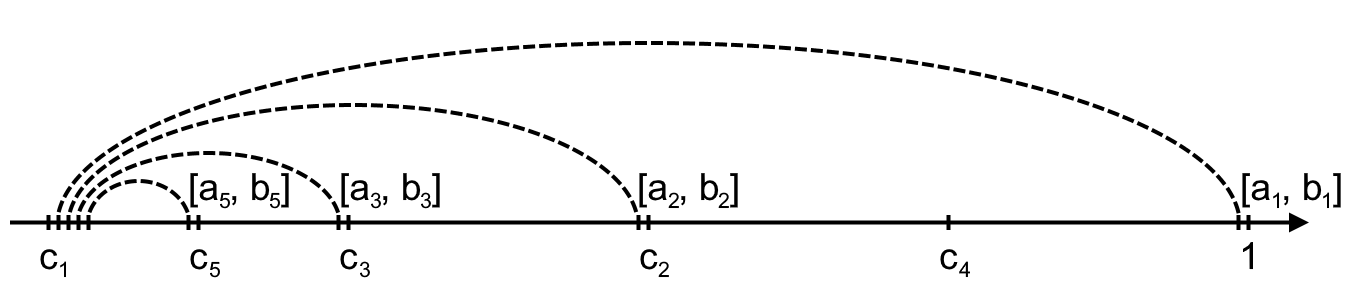
\includegraphics[width=0.80\textwidth, draft=false]{interval-left}
\centering
\caption{последовательность вложенных отрезков для $C[0, 1]$}
\label{fig:interval-left}
\end{figure}

Рассмотрим подпоследовательность $C[0, 1]$ из элементов $c_1, c_{2^k + 1}$
\begin{align}
\begin{split}
c_1 &= 0.100000000\ldots\\
c_2 &= 0.010000000\ldots\\
c_3 &= 0.001000000\ldots\\
c_5 &= 0.000100000\ldots\\
c_9 &= 0.000010000\ldots\\
c_{17} &= 0.000001000\ldots\\
&\ldots
\end{split}
\end{align}

Она ограничивает сверху последовательность отрезков $[a_n, b_n]$, то есть $0 < a_n$ и $b_n < c_{2^k + 1}$ для любого $n \geq 2^k + 1$. Значит в силу свойств пределов последовательностей \cite{matan-limit-properties}:
\begin{equation}
0 < \lim_{n\to\infty} a_n \leq \xi \leq \lim_{n\to\infty} b_n \leq \lim_{k\to\infty} c_{2^k + 1}
\end{equation}

Заметим, что $\lim_{k\to\infty} c_{2^k + 1} = \lim_{k\to\infty} 2^{- k - 2} = 0$, но в таком случае, в силу единственности предела \cite{matan-limit-properties} $\lim_{n\to\infty} a_n = \lim_{n\to\infty} b_n = \xi = 0$, но точка $0$ это первый элемент последовательности $C[0, 1]$. Таким образом, последовательность вложенных отрезков может оказаться внутри последовательности вложенных интервалов, пересечение которых пусто. Следовательно последовательность отрезков удовлетворяющая требованиям доказательства может не существовать, поскольку не существует ни одной точки, которая могла бы принадлежать их пересечению. Конечно современная математика может оперировать и неархимедовыми полями, например, полем гипервещественных чисел в рамках инфинитезимального анализа, однако, благодаря принципу переноса подобные построения не способны дать результатов отличных от результатов полученных с использованием стандартных объектов \cite{infinitesimal-transfer-principle}. 

То есть, без задания правил выбора граничных точек, мы не можем гарантировать того, что строящаяся последовательность отрезков, не окажется ''зажатой'' последовательностью вложенных интервалов имеющих пустое пересечение, а если мы предполагаем бесструктурность бесконечности, то $C[0, 1]$ естественным образом переходит в $U[0, 1]$, где все последовательности вложенных интервалов будут иметь пустое пересечение. Более того, в силу теорем 2 из статьи ''Несчётность множества континуум, шах'' любое вещественное число может быть представлено монотонной последовательностью из $C[0, 1]$, но в этой же статье было показано, что множество таких последовательностей (возможных диагональных построений) оказывается счётным в потенциально бесконечном смысле. Таким образом, множество точек $L[0, 1]$, которые оказываются зажатыми вложенными интервалами элементов $C[0, 1]$, является счётным, равно как и объединение $C[0, 1] \cup L[0, 1]$ \cite{matan-countable-union}. Но в случае множества $C[0, 1] \cup L[0, 1]$ любая последовательность вложенных интервалов имеет пустое пересечение, принципиально исключая любую возможность построения последовательности вложенных отрезков. Таким образом, чтобы данное доказательство работало в потенциально бесконечном случае, нам необходимо, чтобы наша индукция ''знала'' о некоторой ограниченной форме бесконечности, а не упиралась в бесструктурную сущность, которая делает построение противоречивым. При этом принцип вложенных отрезков не нарушается, мы в самом деле можем гарантировать, что если дана бесконечная последовательность вложенных отрезков, то их пересечение не пусто. Но мы не можем гарантировать, что такая последовательность может быть построена под воздействием внешних правил. Иными словами, имея потенциально бесконечную процедуру перечисляющую все точки отрезка, невозможно определить потенциально бесконечную процедуру задающую последовательность вложенных отрезков из точек исходной процедуры. Данный факт ничему не противоречит, если наш выбор не ограничивает внешняя процедура, то мы легко строим последовательности вложенных отрезков имеющие не пустое пересечение. Именно поэтому, нам требуется уйти от описания бесконечности как процесса, исключив взаимодействие бесконечных процедур из уравнения. Однако, когда мы актуализируем бесконечность, то есть воспринимаем бесконечные конструкцию как данность, чтобы доказательство было корректным, нам требуется неочевидное предположение, что существует ограниченная форма бесконечности описывающая количество элементов в последовательности, обладающая ограниченным свойством подобия своей части. Нам требуется обоснованность перехода от любого элемента множества ко всем элементам, даже в рамках современной теории множеств данный переход не всегда очевиден, поскольку мы основываем индукцию на аксиоме бесконечности, которая сама по себе неоднозначна. Значит нам требуются конструктивные доказательства способные обосновать корректный выбор интервалов с демонстрацией того, что их пересечение не пусто. В общем же случае, доказательство вызывает сомнения: мы делаем предположение, после чего, утверждаем существование отображения заданного несовместимыми условиями, приходим к противоречию, которое относим к исходному предположению. 

Примечательно, что если пристально приглядеться к тому, что происходит в доказательстве в случае, когда мы используем только концепцию потенциальной бесконечности, то не сложно видеть, проявление импредикативности понятия всех элементов, которое также связано с неограниченной рефлексивностью актуальной бесконечности на множестве $U[0, 1]$. В самом деле, вещественные числа в мире потенциальной бесконечности являются классами эквивалентности бесконечных последовательностей, предел разности которых равен 0. Принцип вложенных отрезков утверждает, что есть как минимум один класс эквивалентности между последовательностью вложенных отрезков, иными словами, что $\exists c_n: a_n \leq c_n \leq b_n \forall n \in N$. Таким образом, в доказательстве мы пытаемся утверждать, что последовательность $x_n$ не может быть счётной, так как существует подпоследовательность $[a_k, b_k]$ ограничивающая подпоследовательность $c_k$, где $k > n$. То есть, мы в буквальном смысле пытаемся утверждать, будто множество натуральных чисел несчётно, так как в нём можно выделить подпоследовательность $n_i > n$ (снова нам требуются различные формы бесконечности). Обратим внимание, также, на тесную связь противоречия возникающего в доказательстве с аксиомой непрерывности вещественных чисел. С данной аксиомой второго порядка ассоциируется ряд любопытных наблюдений, которые мы рассмотрим далее. В частности, если мы примем аксиому непрерывности (в логике первого порядка) на множестве рациональных чисел, фактически постулируем, что множество рациональных чисел замкнуто по своим пределам, мы конечно получим весьма странную математику данных объектов, но для них приведённое выше доказательство будет работать. Иными словами, аксиома принятая для множества способна изменить его мощность, что весьма странно, тем не менее, это единственная возможность согласовать полученную конструкцию с теоремой о единственности поля вещественных чисел \cite{matan-rational-uniqueness}. Обратим внимание, что дело здесь именно в замыкании, мы от потенциально бесконечного описания, где концепция всех элементов импредикативна, переходим в актуально бесконечное, утверждая существование гипер-рациональных чисел. Но если мы предполагаем, что для полноценного описания реальности нам не нужна потенциальная бесконечность, а нужны лишь актуально бесконечные объекты, то эффекты потенциально бесконечных объектов должны так или иначе воспроизводится в нашей теории, в противном случае мы не можем претендовать на универсальность нашего описания.

Мы снова подтвердили наш вывод о том, что не все потенциально бесконечные процедуры имеют продолжение в области актуальной бесконечности. Настоящего наблюдения более чем, достаточно, для того чтобы утверждать, что данное доказательство в приведённой формулировке математически недостоверно без дополнительных предположений, однако, давайте продвинемся немного дальше. При доказательстве теоремы 2 мы видели, что для любого вещественного числа $r \in [0, 1]$ множество $C[0, 1]$ содержит последовательность $\{c^{rb}_n\}$, являющуюся нижним двоичным приближением числа $r$, также легко показать, что для всех $r \in [0, 1]$ кроме 1 множество $C[0, 1]$ содержит последовательность $\{c^{ru}_n\}$, являющуюся верхним двоичным приближением числа $r$. Таким образом, для любого вещественного числа $r \in [0, 1]$ последовательности интервалов $(c^{rb}_n, r)$ и $(r, c^{ru}_n)$ образованные его нижним и верхним двоичными приближениями имеют пустое пересечение. Заметим, что даже в рамках современного формализма счётное множество $C[0, 1]$ существует как реальный объект. Среди вещественных чисел $r \notin C[0, 1]$ есть счётное множество алгебраических чисел \cite{matan-algebraic-numbers}, объединив их с множеством $C[0, 1]$, которое на самом деле является подмножеством алгебраических чисел, мы получаем счётное множество \cite{matan-countable-union}. Для такого объединения единственной возможностью существования последовательности вложенных отрезков, необходимой для доказательства, является сходимость такой последовательности к какому-либо трансцендентному числу, поскольку все остальные возможности исключены пустыми пересечениями последовательностей интервалов в окрестностях любого числа, кроме трансцендентного. Следовательно, даже если в какой-то момент одна из границ отрезка станет трансцендентным числом, к которому мы будем приближать сколь угодно близко вторую границу, заключение доказательства полностью зависит от предположения несчётности множества трансцендентных чисел. Действительно, если это множество счётно, то предложенная в доказательстве процедура принципиально неосуществима, в противном случае факт несчётности уже доказан. Более того, среди пределов диагональных последовательностей множества $C[0, 1]$, имеются трансцендентные числа, множество таких пределов счётно, а также нам пока неизвестно ни одного вещественного числа, которое бы не принадлежало данному множеству, следовательно если таким образом можно получить все трансцендентные числа, то их множество гарантировано счётно. 

Интересно, что если переформулировать задачу в терминах теории игр, то неопределённость в доказательстве становится более наглядной. Действительно, пусть игроки $A$ и $B$ соревнуются друг с другом по следующим правилам. Задан отрезок $[0, 1]$, первым ходит игрок $A$ он выбирает произвольную точку на данном отрезке. Следующим ходом игрок $B$ выбирает две точки, но с условием, что отрезок соединяющий их не пересекает ни одну из существующих точек выбранных игроком $A$. Затем, снова ходит игрок $A$ и выбирает другую произвольную точку (ему нельзя выбирать одну и ту же точку дважды). Дальше опять ходит игрок $B$, он выбирает две любые точки на отрезке выбранном на предыдущем ходу, с тем же требованием, чтоб между ними не лежало ни одной точки игрока $A$ и т.д. Игра длится потенциально бесконечное время, побеждает тот игрок у которого осталось больше доступных ходов. Ясно, что игрок $B$ всегда должен выбирать 2 точки, и не может выбрать одну, иначе игрок $A$ одним из следующих ходов выберет эту точку и игрок $B$ проиграет, так как у него не останется ходов. Тогда, множество вещественных чисел на отрезке $[0, 1]$ является детерминированным для данной игры, то есть у одного из игроков есть выигрышная стратегия. Действительно если игрок $A$ будет выбирать точки из последовательности $C[0, 1]$, то при стремлении количества ходов к бесконечности он разобьёт отрезок $[0, 1]$ на множество интервалов, каждый из которых либо пустой, либо содержит ровно одну точку (здесь нам не важно какому числу она соответствует рациональному, алгебраическому или трансцендентному, из предположения, что она не одна следовало бы существование ещё как минимум одной точки с ненулевым расстоянием до первой, не разделённым элементом $C[0, 1]$, что свидетельствовало бы о конечности $C[0, 1]$). Но это означает, что у игрока $B$ не осталось ходов, поскольку ему требуется как минимум две точки не разделанные точками поставленными игроком $A$, в то время как $A$ ещё может делать ходы, выбирая оставшиеся точки. Любопытно, что при стремлении количества ходов к бесконечности, у игрока $A$ уже появляется преимущество, в то время, как доказываемая нами теорема, утверждает, что победить должен игрок $B$. Чтобы гарантировать результат теоремы, нам требуется изменить правила игры, если заканчивается время определяющее некоторую форму бесконечности, иными словами, без вмешательства в сам игровой процесс, мы не можем обеспечить победу игроку $B$.

Возможно, данную игру можно каким-то образом модифицировать и разрешить игроку $B$ выбирать одну точку, сформулировав условие победы, так что оставшееся трансцендентное число делает его победителем. Присмотревшись к последовательности точек, которые выбирает игрок $B$, а именно к их двоичной записи, можно заметить, что с каждым следующим ходом все большее и большее количество значащих двоичных цифр фиксируется и не изменяется с последующими ходами. Тоже самое происходит с ходами игрока $A$, если мы рассмотрим последовательность выбранных им чисел, которые непосредственно ограничивают доступное пространство для игрока $B$. Словно оба игрока на каждом ходу выбирают некоторое натуральное число и используют его двоичную запись, чтобы зафиксировать новый набор цифр, начинающийся с последней зафиксированной на предыдущем ходу цифры. Если $B$ построит трансцендентное число, то есть число не принадлежащее множеству, являющемуся объединением множества $C[0, 1]$ и множества алгебраических чисел, то он выигрывает, в противном случае выигрывает игрок $A$. Но это очень похоже на классическую игру, при помощи которой сформулирована аксиома детерминированности \cite{determinacy}, справедливость которой означает и верность континуум-гипотезы \cite{cantor-countinuum-hypothesis}. Иными словами, поиск стратегии для игрока $B$ позволяющей строить трансцендентные числа для любой стратегии игрока $A$ может оказаться совсем непростой задачей. 

Переформулировка в терминах теории игр, на взгляд авторов, делает проблему описания бесконечности более наглядной, позволяя детально рассмотреть смысл предположений, которые мы делаем относительно данной сущности. В самом деле, для победы игрока $B$ бесконечность должна обладать свойством уникальности (эталонности) - то есть совокупность предшествующих ей чисел должна быть воспроизводимой (одинаковой для любого множества - универсальной) и все они должны быть конечными индуктивными объектами теории (тотальность индукции). Тогда даже если игрок $A$ способен бесконечным количеством ходов исключить все вещественные числа, игрок $B$ не может проиграть где-то на полпути, ведь это будет означать, что он проиграл на конечном ходе, что противоречит непрерывности вещественных чисел. Несложно видеть, что такую уникальность в рамках современной интерпретации обеспечивает аксиома регулярности, запрещающая бесконечные убывающие цепочки и позволяющая утверждать, что наше определение минимального трансфинитного числа обозначает реальный объект, в отличии, например, от определения максимального натурального числа, которое не обозначает никакого объекта теории. Таким образом, аксиома регулярности закрепляет наше предположение, что среди систем вполне упорядоченных объектов не имеющих максимум существуют системы, которые допустимо называть минимальными. Тем самым оставляя за пределами теории системы, описываемые альтернативным предположением, что какой бы ни была такая система, всегда найдётся подсистема также не имеющая максимума (которая могла бы соответствовать бесконечному количеству ходов игрока $B$ до его проигрыша). В то же самое время, бесконечное количество ходов содержит как чётные ходы так и нечётные, совокупностям которых не может соответствовать ни одно конечное число, значит, с одной стороны бесконечность неделима на две бесконечные части, с другой она может быть разделена на две бесконечные части. К обсуждению того, как такая комбинация свойств становится необходимой и возможной в рамках современной интерпретации теории множеств, мы вернёмся в следующих статьях настоящей серии.

Обратимся теперь к оригинальному доказательству Кантора 1879 года \cite{cantor-original}. Рассмотрим непрерывный интервал $(0, 1)$. Если бы данное многообразие было бы счётным, то должна была бы существовать просто бесконечная последовательность $x_1, x_2, \dots, x_n, \dots$, состоящая из всех действительных чисел $\geq 0$ и $\leq 1$ и такая, что всякое число $y$ из этого интервала занимало бы определённое место в этой последовательности. Этому однако противоречит весьма общая теорема.

Теорема: {\sl Если имеется просто бесконечная последовательность неравных вещественных чисел $x_1, x_2, \dots, x_n, \dots$, заданная по какому-либо закону, то во всяком данном интервале $(a, b)$ можно указать число $y$ (а значит, и бесконечно много таких чисел), которое не содержится в этой последовательности (как её член).}

Доказательство: 

Обозначим исходную последовательность за $P$. Возможны два случая:

\begin{enumerate}
    \item Прежде всего замечаем, что если наше многообразие $P$ не является всюду плотным в интервале (здесь всюду плотность означает наличие точек $P$ в любом сколь угодно маленьком подинтервале, по сути плотный порядок в современных терминах), то внутри этого интервала должен существовать другой интервал $(c, d)$, все числа которого не принадлежат $P$; тогда в качестве $y$ можно брать любое число интервала $(c, d)$; оно расположено в интервале $(a, b)$ и определённо не содержится в нашей последовательности $P$. Остаётся единственный и более трудный случай.
    \item Пусть многообразие $P$ всюду плотно в интервале $(a, b)$. В этом случае всякий сколь угодно малый интервал $(c, d)$, расположенный в $(a, b)$, содержит числа нашей последовательности $P$. Так как в нашей последовательности определённо имеются числа, содержащиеся внутри интервала $(a, b)$, то одно из них должно иметь наименьший индекс, скажем $x_{k_1}$, а некоторое другое число $x_{k_2}$ должно быть с непосредственно большим индексом. Обозначим меньшее из двух чисел $x_{k_1}$, $x_{k_2}$ через $a_1$, а большее через $b_1$ (их равенство исключается, так как мы предположили, что наша последовательность состоит из различных чисел). Тогда по определению 
\begin{align}
\begin{split}
a < a_1 &< b_1 < b\\
k_1 &< k_2
\end{split}
\end{align}

Кроме того, следует заметить, что все числа $x_m$ нашей последовательности, для которых $m < k_2$, не находятся внутри интервала $(a_1, b_1)$, что непосредственно вытекает из определения чисел $x_{k_1}$, $x_{k_2}$. Совершенно так же можно рассмотреть два числа $x_{k_3}$, $x_{k_4}$ нашей последовательности, которые попадают внутрь интервала $(a_1, b_1)$ и меньшее из них будет обозначено через $a_2$, а большее - через $b_2$. Тогда имеем
\begin{align}
\begin{split}
a_1 < a_2 &< b_2 < b_1\\
k_2 < k_3 &< k_4
\end{split}
\end{align}

и очевидно, что все числа $x_m$ нашей последовательности, для которых $m < k_4$, не попадают внутрь интервала $(a_2, b_2)$. После того как, следуя тому же закону, получим интервал $(a_{n - 1}, b_{n - 1})$, оказывается, что следующий интервал получается из него тем, что находим два первых (т. е. взятых с наименьшими индексами) числа нашей последовательности $P$ (пусть они будут $x_{k_{2n - 1}}$ и $x_{k_{2n}}$), которые попадают внутрь интервала $[a_{n - 1}, b_{n - 1}]$; меньшее из этих чисел будет обозначаться через $a_n$, а большее - через $b_n$.

Тогда интервал $(a_n, b_n)$ расположен внутри всех предшествующих интервалов и находится к нашей последовательности $P$ в том своеобразном отношении, что все числа $x_m$, для которых $m \leq 2n$, определённо расположены вне него. Так как, очевидно
\begin{align}
\begin{split}
a < a_1 < a_2 < \dots < a_{n - 1} < a_n &< b_n < b_{n - 1} < \dots < b_2 < b_1 < b\\
k_1 < k_2 < &\dots < k_{2n - 1} < k_{2n}
\end{split}
\end{align}

Поскольку числа $k_1, k_2, \dots, k_{2n - 1}, k_{2n}$, будучи индексами, являются целыми числами, то $k_{2n} \geq 2n$, а потому $n < k_{2n}$; мы можем поэтому определённо сказать - и этого для последующего достаточно, что если $n$ - произвольное целое число, то величина $x_n$ расположена вне интервала $(a_n, b_n)$. Продолжая описанную процедуру неограниченно долго можно установить следующее.

Так как числа $a_1, a_2, a_3, \dots, a_n, \dots$, возрастают по величине, будучи, однако, заключёнными в интервале $(a, b)$, то по известной основной теореме учения о величинах они имеют определённый предел, который мы обозначим через $A$, так что $\lim_{n\to\infty} a_n = A$. То же самое справедливо для чисел $b_1, b_2, b_3, \dots, b_n, \dots$, которые убывают и притом тоже расположены в интервале $(a, b)$; их предел мы обозначим через $B$, так что $\lim_{n\to\infty} b_n = B$. Очевидно, что 
\begin{equation}
a_n < A \leq B < b_n
\end{equation}

Но легко видеть, что случай $A < B$ представиться не может, так как в противном случае всякое число $x_n$ нашей последовательности было бы расположено вне интервала $(A, B)$, ибо $x_n$ находится вне интервала $(a_n, b_n)$; тогда, вопреки предположению, наша последовательность не была бы всюду плотной в интервале $(a, b)$.

Остаётся поэтому лишь случай $A = B$, а тогда оказывается, что число $y = A = B$ не принадлежит нашей последовательности $P$. Действительно, если бы оно было членом нашей последовательности, например $n$-м, то имели бы $y = x_n$. Последнее же равенство невозможно ни для какого значения $n$, так как $y$ расположено внутри интервала $(a_n, b_n)$, а $x_n$ вне его.

\end{enumerate}

Теорема доказана.

В доказательстве Кантора, речь уже идёт о последовательности вложенных интервалов, а не отрезков, явно строящихся на основе подпоследовательностей забегающих вперёд исходной последовательности $n_i > n$, пересечение которых по построению не должно быть пустым. Смысл рассуждений сводится к тому, что мы, располагая некоторой последовательностью вещественных чисел, задаём правила построения двух подпоследовательностей, неизбежно указывающих на число или множество чисел, которые не могут содержатся в данной последовательности. Однако аргументация, того что предложенный набор правил корректен для всех возможных исходных последовательностей, отсутствует, что не может не настораживать, ведь как мы уже отмечали, попытка сконструировать бесконечную процедуру, забегая вперёд другой бесконечной процедуры, не всегда приводит к построению существующего в области актуальной бесконечности объекта и зависит от предполагаемой структуры бесконечности. Отметим, что для Кантора противопоставление актуальной и потенциальной бесконечности в доказательстве, по мнению авторов, играет ключевую роль. В самом деле, в первой версии доказательства, он обозначает предельные элементы как $\alpha^{\infty}$ и $\beta^{\infty}$, но предполагает, что последовательность не может содержать элемент с подобным индексом, в то время как сам актуально бесконечный элемент существует как фиксированная точка, а не как абстрактный образ направления последовательности. В отличии от более зрелого диагонального построения, Кантор аккуратно не анализирует границы импредикативного существования образа, где понятие всех элементов последовательности не определено, и предикативного существования фиксированной точки заданной как абсолютно бесконечный объект. Что не позволяет ему в сформулировать предположения необходимые для корректности доказательства в явном виде. Без таких предположений классы эквивалентности последовательностей $\alpha^{\infty}$ и $\beta^{\infty}$ вполне могут оказаться состоящими из подпоследовательностей $P$, представляя собой просто некоторую аннотацию этого объекта. 

Интуитивно Кантор стремится придать трансцендентным точкам ту же реальность, которой наделены рациональные или алгебраические числа. Однако, в таком случае необходимо аргументировать почему бесконечные элементы $\alpha^{\infty}$ и $\beta^{\infty}$ не могут завершать бесконечную последовательность, или почему количество элементов подпоследовательности не может быть тождественно бесконечному количеству элементов всей последовательности, позволяя предельным точкам иметь позиции, не имеющие образа среди позиций элементов подпоследовательностей определяющих эти предельные точки (нет биекции при рассмотрении $a_1, a_2, a_3, \dots, a_n, \dots$ как подпоследовательности, но есть при рассмотрении как самостоятельной последовательности, то что мы наблюдаем в случае натурального ряда и чётных чисел). Возможно, именно сознание того факта, что для корректной интерпретации данного доказательства требуется целостная система предположений и подтолкнула Кантора к разработки соответствующей теории. Несложно заметить, что в случае актуально бесконечного множества $U[0, 1]$ с бесструктурной морфологией доказательство не работает, поскольку в силу теоремы 3 точка $A = B$ принадлежит множеству $U[0, 1]$, а значит искомая последовательность отрезков не может существовать, так как отсутствует такая точка, которая в соответствии с требованиями доказательства могла бы ей принадлежать. Это можно рассматривать через проблему интерпретации взаимно однозначного соответствия, сильная интерпретация означает биекцию между индексами последовательности и индексами подпоследовательностей задающих систему вложенных интервалов, что делает доказательство корректным, в то время как, слабая позволяет существовать элементам последовательности $P$ не имеющим образа в бесконечном множестве построенных интервалов. Снова сделаем оговорку, что формальное определение множества $U[0, 1]$ довольно расплывчато, поскольку опирается лишь на предположение о возможности бесконечных математических процедур, чтобы под этим не подразумевалось, тем не менее, оно точно демонстрирует необходимость дополнительных предположений для того, чтобы доказательство работало. В свою очередь, множество $C[0, 1]$ раскрывает суть находки Кантора: если задана бесконечная последовательность элементов некоторого дискретного (не непрерывного) упорядоченного всюду плотного множества, то существует алгоритм построения подпоследовательностей однозначно идентифицирующих определённый разрыв или сечение данного множества. В частности, данный алгоритм может быть использован для получения различных классов трансцендентных чисел. 

Рассмотрим ход доказательства более детально. Мы исследуем два случая: если последовательность не всюду плотна, то мы с лёгкостью находим множество точек не принадлежащих исходной последовательности, если же последовательность всюду плотна, то мы начинаем строить бесконечную последовательность интервалов. Выбираем произвольный интервал $(a, b) \in [0, 1]$ и находим два числа $x_{k_1}$ и $x_{k_2}$ с наименьшими индексами $k_1$ и $k_2$ попадающие в интервал $(a, b)$, обозначив меньшее из них через $a_1$, а большее через $b_1$. Далее, мы повторяем процедуру с интервалом $(a_1, b_1)$, получаем новый интервал $(a_2, b_2)$, который в свою очередь подвергаем той же процедуре, получая в итоге бесконечную последовательность вложенных интервалов $\{(a_n, b_n)\}$. Доказательство продолжается установлением пределов последовательностей $\lim_{n\to\infty} a_n = A$ и $\lim_{n\to\infty} b_n = B$, и далее демонстрацией того, что выстроенная конструкция возможна только при равенстве этих пределов $A = B$.

Однако, перейдя к пределам в доказательстве мы вспоминаем об индексе. Утверждается, что число $y = A = B$ не может принадлежать исходной последовательности, так как противное предположение, что $y = x_{n} \in P$ наталкивается на противоречие, ведь $y$ определённо принадлежит интервалу $(a_n, b_n)$, а $x_n$ - определённо нет. Проблема только в том, что предположение, что $y = x_{n}$ моментально обрушивает всю тщательно выстроенную конструкцию вложенных интервалов, ещё до того, как у нас появляется возможность получить интервал $(a_n, b_n)$, чтобы проверить принадлежность ему значений $y$ и $x_n$. Действительно, если $x_n = A$, то никакого интервала $(a_n, b_n)$ в принципе существовать не может, так как $a_n = x_{k_{2n - 1}}$, где $n < k_{2n - 1}$, то есть мы должны найти $a_n$ в последовательности $P$ где-то после $x_n$, однако в последовательности $P$ нет ни единого элемента после $x_n$, который мог бы одновременно быть больше $x_n$, чтобы исключить его из интервала, и быть меньше либо равным $A$, как пределу последовательности, элементом которой он является. Значит противоречие возникло с несуществующим интервалом, и неудивительно, что какой-то элемент ему принадлежит и не принадлежит одновременно. Проблема в том, что без строго задания морфологии бесконечности у нас отсутствует предикативный контекст позволяющий определить, когда забегая вперёд $x_n$ мы остаёмся в рамках последовательности $P$, а когда выходим за её пределы. Вследствие чего мы не в состоянии различить, является ли противоречие следствие предположения в доказательстве или обусловлено другим противоречием, которое запрещает существование бесконечной последовательности вложенных интервалов, удовлетворяющей требованиям доказательства для любой исходной последовательности $P$. Такова расплата, за попытку забежать вперёд бесконечной последовательности вне предикативного контекста, - обнаруженные противоречия, затрагивающие элемент с определённым индексом, разрушают все построения основанные на элементах с превосходящим индексом, и не позволяют делать утверждения относительно свойств исходной последовательности. Отметим, что в нашем исследовании мы снова и снова сталкиваемся с трудностями, вызванными вольным использованием понятия бесконечность и процедур связанных с ним, это чрезвычайно важное наблюдение, так как по какой-то причине мы считали, что можем приписывать бесконечности произвольные свойства, не утруждая себя их исследованием и строгим определением, но оказывается, что зависимые бесконечные процедуры существенно ограничены теми процессами, от которых они зависят. Здесь уже становится понятно, что доказательство как и его аналог разобранный ранее использует внутренне неконсистентные условия построения, которые можно оправдать только довольно специфичными предположениями относительно структуры бесконечных объектов, заведомо подразумевающие ограничение импредикативности связанной с рефлексивностью. Именно к этому, в конечном итоге, приходит Кантор, филигранно разделивший полиномиальную и экспоненциальную области в порядковых типах, так что первая остаётся рефлексивной, в то время как вторая становится полностью предикативной, на чём мы остановимся в следующих статьях серии. Давайте попробуем немного углубиться в обнаруженную проблему и выяснить какие свойства исходной последовательности $P$, могут приводить к тому, что невозможно построить сразу две бесконечных монотонных подпоследовательности $\{a_n\}$ и $\{b_n\}$, ограничивающих друг друга и имеющих общий предел не являющийся их элементом. Не сложно сообразить, что это свойство непрерывности \cite{matan-completeness}.

До того как мы начали доказывать данную теорему у нас не было никаких оснований утверждать, что все элементы непрерывного множества не могут быть представлены в виде бесконечной последовательности, в самом деле, множество натуральных чисел в определённой степени тоже непрерывно, ведь между двумя последовательными натуральными числами не может существовать ещё одно. Тогда, не совсем понятно, на каком основании мы не рассматриваем в доказательстве случай последовательности элементов некоторого непрерывного множества. Ведь, на такой последовательности принципиально невозможно построить последовательность вложенных интервалов содержащих в своём пересечении хотя бы одну точку, что следует из довольно общей теоремы.

Теорема 2: {\sl Если имеется бесконечная последовательность неравных элементов $x_1, x_2, \dots, x_n, \dots$, заданная по какому-либо закону, где все элементы связаны между собой отношением порядка, то не может существовать пара бесконечных подпоследовательностей, определяемая некоторым законом удовлетворяющим следующим требованиям: элементы выбираются попарно и не равны между собой, элементы первой пары произвольны, оба элемента каждой следующей пары, подчиняют меньший элемент и не превосходят больший элемент предыдущей пары и имеют наименьший возможный индекс в исходной последовательности, такая (пара) что исходная последовательность содержит непустое множество элементов, каждый из которых подчиняет меньший элемент и не превосходит больший элемент любой пары элементов этих подпоследовательностей.}

Доказательство:

Обозначим исходную последовательность за $P$. Поскольку все элементы последовательностей согласно условию не равны между собой, то не строгое отношение порядка обращается в строгое. Согласно требованиям закона построения пары бесконечных подпоследовательностей мы выбираем произвольным образом два первых элемента $x_{k_1}$ и $x_{k_2}$ последовательности $P$, где $k_1 < k_2$, обозначим меньший из них за $y_1^-$, а больший за $y_1^+$, один из них становится элементом одной подпоследовательности, второй - другой. Далее мы снова выбираем пару элементов $x_{k_3}$ и $x_{k_4}$, где $k_3 < k_4$, обозначив меньший из них за $y_2^-$, а больший за $y_2^+$, в силу требований закона они имеют наименьшие возможные индексы $k_3$ и $k_4$ в последовательности $P$ и удовлетворяют соотношениям $y_1^- < y_2^-$, $y_1^- < y_2^+$, $y_2^- < y_1^+$ и $y_2^+ < y_1^+$, откуда пользуясь транзитивностью отношения порядка имеем:
\begin{align}
\begin{split}
y_1^- < y_2^- &< y_2^+< y_1^+\\
k_1 < k_2 &< k_3 < k_4
\end{split}
\end{align}

Соответственно, достигнув пары $y_{n - 1}^-$ и $y_{n - 1}^+$, следуя тем же требованиям закона, мы выбираем очередную пару элементов $x_{k_{2n - 1}}$ и $x_{k_{2n}}$ с наименьшими возможными индексами $k_{2n - 1}$ и $k_{2n}$, где $k_{2n - 1} < k_{2n}$, обозначаем меньший из них за $y_n^-$, а больший за $y_n^+$, в результате чего пользуясь транзитивностью отношения порядка получаем:
\begin{align}
\begin{split}
y_1^- < y_2^- < \dots < y_{n - 1}^- < y_{n}^- &< y_{n}^+ < y_{n - 1}^+ < \dots < y_2^+< y_1^+\\
k_1 < k_2 < k_3 &< \dots < k_{2n - 1} < k_{2n}
\end{split}
\end{align}

Предположим, что утверждение теоремы не верно, и процесс формирования подпоследовательностей мы можем продолжать бесконечно, при этом существует некоторое не пустое множество элементов $T$ последовательности $P$ такое, что все $t \in T$ обладают свойством $y_{l}^- < t < y_{l}^+$, для всякого $l = 1, 2, 3, \dots$. Поскольку все элементы множества $T$ являются элементами последовательности $P$, то все они имеют в ней какой-то индекс, значит среди этих элементов непременно есть элемент с наименьшим индексом $m$, обозначим его $z = x_m$. Тогда в силу нашего предположения возможны всего 3 случая:

\begin{enumerate}
    \item $m = k_{2n - 1}$ или $m = k_{2n}$, то есть $z$ является одним из элементов пары $\{y_{n}^-, y_{n}^+\}$, и следовательно элементом одной из последовательностей, другими словами либо $z = y_{n}^-$, либо $z = y_{n}^+$. Однако, это противоречит тому, что элемент $z$ принадлежит множеству $T$, и для него как для любого элемента множества $T$ должно выполнятся условие $y_{l}^- < z < y_{l}^+$ для всякого $l = 1, 2, 3, \dots$, в частности для $l = n$ имеем $y_{n}^- < z < y_{n}^+$.
    \item $k_{2n - 2} < m < k_{2n - 1}$, то есть $z$ расположен между какими-то парами $\{y_{n - 1}^-, y_{n - 1}^+\}$ и $\{y_{n}^-, y_{n}^+\}$. Но, это противоречит требованиям закона о выборе элементов с наименьшим возможным индексом в последовательности $P$, ведь элемент $z$ удовлетворяет условию: $y_{n - 1}^- < z < y_{n - 1}^+$, но при этом имеет индекс $m < k_{2n - 1} < k_{2n}$ , значит мы должны были выбрать именно его в качестве одного из двух элементов пары $\{y_{n}^-, y_{n}^+\}$.
    \item $k_{2n - 1} < m < k_{2n}$, то есть $z$ расположен между элементами какой-то пары $\{y_{n}^-, y_{n}^+\}$. Однако, мы снова приходим к противоречию с требованиями закона о выборе элементов с наименьшим возможным индексом в последовательности $P$, ведь элемент $z$ удовлетворяет условию формирования подпоследовательностей: $y_{n - 1}^- < z < y_{n - 1}^+$, но при этом имеет индекс $m < k_{2n}$, таким образом мы были обязаны выбрать именно его в качестве второго элемента пары $\{y_{n}^-, y_{n}^+\}$.
\end{enumerate}

Следовательно, никоим образом мы не можем согласовать наше предположение с требованиями закона формирования пары подпоследовательностей, что может означать только то, что оно не верно. Теорема доказана.

Теорема, несмотря на свою своеобразность, подобно теореме 1, позволяет установить, что построение Кантора в общем случае является неконсистентным, а его доказательство оказывается корректным лишь при исходном разделении форм бесконечности. Данное обстоятельство открывает любопытную перспективу для интерпретации истории создания теории множеств. В конечном итоге Кантор выстраивает арифметику порядковых типов, которая сохраняет свойство рефлексивности в полиномиальной области, однако в экспоненциальной области становится предикативной. Именно это обеспечивает корректность рассматриваемого доказательства для всех экспоненциальных и более сложных моделей вещественных чисел. Иными словами, исходное доказательство Кантора оказывается сравнительно слабым с точки зрения ключевой для математики задачи очерчивания границ применимости. Оно требует специфических предположений о морфологии бесконечности - универсальности, тотальности и экспоненциально ограниченной рефлексивности, формулировке которых Кантор посвятил внушительную часть своих исследований. Это наблюдение о мотивах Кантора несколько смягчает тот идеализированный образ, который мог бы сложиться при чтении настоящей серии статей вследствие его несравненно более глубокого и концептуального понимания предмета, нежели современная упрощённая интерпретация.

Теорема 2 справедлива для любых объектов, к которым применимо отношение порядка, в частности - для вещественных чисел. Представляет интерес применение данной теоремы к различным множествам. Так, если из множества $C[0,1]$ исключить некоторый элемент, то, подобрав первую пару элементов, можно построить бесконечные последовательности, пределы которых равны исключённому элементу. Если же никакие элементы не исключаются, последовательности могут сходиться как к иррациональным числам, так и к рациональным числам, имеющим бесконечную двоичную запись. На множестве рациональных чисел такие последовательности сходятся к иррациональным числам, а на множестве алгебраических чисел - к трансцендентным. Добавляя к множеству алгебраических чисел известные счётные множества трансцендентных чисел, можно получать последовательности, сходящиеся к новым классам трансцендентных чисел. Однако при рассмотрении произвольных множеств всегда остаётся справедливым утверждение, что пересечение интервалов, образованных построенными подпоследовательностями, никогда не содержит элементов исходной последовательности. Если же принять аксиому непрерывности для множества $C[0,1]$, фактически предположив, что не существует вещественных чисел, отличных от перечисленных в данном множестве, то всякая последовательность вложенных интервалов, удовлетворяющая критериям описанного построения, оказывается конечной. Она может быть сколь угодно длинной, однако все элементы $C[0,1]$ достижимы за конечное число итераций. То же самое справедливо и для производной последовательности вложенных интервалов, что полностью соответствует определению потенциальной бесконечности.

Попробуем применить данную теорему к множеству $C$, для которого принимается аксиома непрерывности: каковы бы ни были непустые подмножества $A$ и $B$ исходного множества $C$, такие что для любых $a \in A$ и $b \in B$ выполняется неравенство $a \leq b$, существует элемент $c \in C$, удовлетворяющий условию $a \leq c \leq b$ для всех $a \in A$ и $b \in B$ \cite{matan-completeness}. Иными словами, между элементами данного множества не существует никаких других элементов, которые могли бы быть связаны с ними отношением порядка. При наличии лишь аксиом порядка и аксиомы непрерывности невозможно утверждать, что такое множество не может быть представлено в виде последовательности: указанных аксиом явно недостаточно для доказательства или опровержения этого утверждения. Тогда, согласно теореме 2, последовательность $P$ не содержит ни одного элемента, который одновременно превосходил бы минимальный элемент и был бы меньше максимального элемента любой пары элементов бесконечных подпоследовательностей. Этого оказывается достаточно, чтобы разделить множество $P$ на два класса: в первый входят элементы, не превосходящие минимального элемента любой пары, а во второй - элементы, подчиняющие максимальный элемент любой пары. В силу свойств сечений, вытекающих из аксиомы непрерывности, требуется, чтобы либо в первом классе существовал максимальный элемент, либо во втором - минимальный \cite{matan-cut}. Обозначим такой элемент через $\xi$, независимо от того, какому классу он принадлежит. Если $\xi$ принадлежит первому классу, то он обязан входить в одну из последовательностей, то есть являться элементом одной из пар: в противном случае он принадлежал бы множеству $T$, что противоречит теореме 2. Предположим, что $\xi$ действительно имеет некоторый индекс в последовательности $P$ и в соответствующих подпоследовательностях. Тогда хотя бы одна из подпоследовательностей оказывается конечной и заканчивается этим индексом, поскольку по построению все минимальные элементы пар принадлежат первому классу, все элементы которого не превосходят $\xi$; следовательно, для следующей пары минимальный элемент отсутствует. Аналогичное противоречие возникает, если $\xi$ принадлежит второму классу. Таким образом, в силу теоремы 2 для любой последовательности $P$ элементов непрерывного множества не существует пары бесконечных подпоследовательностей, удовлетворяющих условиям теоремы.

Для большей формальности введём ряд определений. Две последовательности элементов линейно упорядоченного множества называются {\it разделяющими}, если любой элемент одной последовательности не превосходит любого элемента другой и любой элемент исходного множества может быть отнесён к одному из двух множеств (классов): элементов, не превосходящих все элементы одной последовательности, и элементов, не подчиняющих все элементы другой последовательности. Иными словами, если найдётся элемент первой последовательности, такой что элемент исходной последовательности его не превосходит, то элемент исходной последовательности относится к первому множеству (классу), если же найдётся элемент второй последовательности подчинённый элементу исходной последовательности, то ко второму множеству (классу). Если все элементы первой последовательности не превосходят всех элементов второй, и не существует элементов исходного множества, которые не относятся к одному из данных классов, то последовательности разделяют множество. То есть последовательности $\{a_n\}$ и $\{b_n\}$ называются {\it разделяющими} множество $M$, если
\begin{equation}
\forall i, j \in \mathbb{N} \; a_i \leq b_j \; \wedge \; \forall m \in M \; \exists n \in \mathbb{N}: (m \leq a_n \; \vee \; b_n \leq m)
\end{equation}

Разделяющие последовательности могут быть как конечными, так и бесконечными. Если при разделении оба множества содержат предельные точки, то обе последовательности могут быть конечными (например, $\{-3, -2, -1\}$ и $\{1, 0\}$ разделяют множество целых чисел). Если, как в случае непрерывных множеств, лишь одно из множеств может содержать предельную точку, то конечной может быть только одна последовательность (например, $\{0\}$ и $\{1/n\}$ разделяют множество действительных чисел). Наконец, в том случае, когда ни одно из множеств не содержит предельной точки, то обе разделяющие последовательности необходимо являются бесконечными (например, $\{3, 178/57, 354/113, 104347/33215, \dots\}$ и $\{22/7, 179/57, 355/113, 104348/33215, \dots\}$ разделяют множество рациональных чисел, имея общим пределом $\pi$). Отметим, что для упрощения, в отличие от последовательностей, фигурирующих в теореме 2, мы требуем, чтобы все элементы одной последовательности не превосходили элементы другой. Легко показать, что на самом деле они должны быть строго меньше: в противном случае элемент принадлежал бы одновременно двум множествам, и последовательности по определению не были бы разделяющими. Таким образом, теорема справедлива для более общего класса последовательностей. С другой стороны, мы не ограничиваемся алгоритмом построения, предложенным в теореме, что делает класс разделяющих последовательностей более широким. Нетрудно показать, что если линейно упорядоченное множество непрерывно, то разделяющие его бесконечные строго монотонные последовательности не могут существовать: одна из них необходимо содержит максимальный или минимальный элемент, который неизбежно завершает эту последовательность. По-видимому, здесь может возникнуть целое направление исследований окрестностей разделения множеств, способствующее более глубокому пониманию понятия непрерывности; возможно даже, что с помощью разделяющих последовательностей удастся сформулировать альтернативную версию аксиомы непрерывности. Однако это выходит далеко за рамки темы настоящей статьи, поэтому мы ограничимся лишь определением, под которое подпадают последовательности, строящиеся в оригинальном доказательстве Кантора. 

Согласно теореме 2, пересечению интервалов, образованных последовательностями $\{a_n\}$ и $\{b_n\}$, не может принадлежать ни одна точка последовательности $P$. Таким образом, мы имеем дело с бесконечными последовательностями, разделяющими множество $P$. Однако по условию $P$ - произвольная последовательность вещественных чисел; в частности, она может содержать все вещественные числа и, следовательно, быть непрерывной. В этом случае по построению искомые подпоследовательности $\{a_n\}$ и $\{b_n\}$ существовать не могут. Для обоснования данного утверждения не требуются даже определение предела и теорема Вейерштрасса о пределе монотонной последовательности, в доказательстве которой, заметим, центральную роль играет аксиома непрерывности \cite{matan-weierstrass}. Это вполне закономерно: в свете изложенного выше утверждение теоремы, доказанной Кантором, может быть интерпретировано как невозможность существования бесконечных разделяющих подпоследовательностей непрерывной последовательности. Если же такие последовательности существуют (например, при аккуратном разделении форм бесконечности), то они действительно обладают пределом, причём этот предел не может быть элементом исходной последовательности, и доказательство работает корректно. В то же время мощности счётного множества $C[0,1]$ достаточно, чтобы получить последовательность интервалов, пересечение которых содержит ровно одну точку или вовсе не содержит точек. Следовательно, в пределе последовательность $\{a_n\}$ в лучшем случае оставляет в пересечении единственную точку, на которую одновременно претендуют последовательность $\{b_n\}$ и сама предельная точка, которая не должна принадлежать ни одной из этих последовательностей. Удовлетворить все эти притязания оказывается невозможным. При ближайшем рассмотрении обнаруженный факт о непрерывных множествах оказывается довольно простым. Аксиома непрерывности, принятая для любого множества, запрещает сечения этого множества типа ''пробел''. Это означает, что как бы мы ни рассекали данное множество на два подмножества, ситуация, при которой в обоих из них имеются счётные подмножества, являющиеся бесконечными последовательностями, стремящимися друг к другу и разделяющими множество, невозможна. Более того, для получения такого заключения достаточно аксиомы, запрещающей лишь сечения типа ''пробел''. Назовём её {\it аксиомой связности}: множество называется {\it связным}, если каково бы ни было его сечение, меньшее подмножество имеет максимум или большее подмножество имеет минимум (в частности, не исключается случай, когда оба утверждения выполняются одновременно).

Например, множество целых чисел связно при естественном упорядочении (это можно принять в качестве аксиомы). Для данного множества не могут существовать разделяющие бесконечные последовательности, но это никак не влияет на мощность множества. Для наглядности упорядочим целые числа следующим образом: $x < y \Leftrightarrow 1/x < 1/y$ при $x \neq 0$ и $y \neq 0$; отрицательные числа считаются меньшими нуля, а положительные - большими. В результате все целые числа могут быть представлены точками внутри отрезка $[-1, 1]$, причём минимальным целым числом оказывается $-1$, а максимальным - $1$. Полученное множество также является связным, и для него бесконечные разделяющие последовательности не существуют. Тем не менее оно остаётся счётным: его элементы могут быть пронумерованы стандартным образом - $0, 1, -1, 2, -2, \dots$. Если мы исключаем точку $0$ из множества оно перестаёт быть связным, и последовательности $1, 2, \dots$ и $-1, -2, \dots$, получаемые из исходной, разделяют его на две части. Даже на множестве натуральных чисел нетрудно задать порядок, при котором чётные числа представляются точками полуинтервала $[-1, 0)$, а нечётные - полуинтервала $(0, 1]$.  Такой порядок отчётливо демонстрирует эффект полноты множества: полученные множества полны в точке $0$. Более того, в этой точке они становятся импредикативными: между ближайшим к нулю элементом и самим нулём всегда существуют ещё более близкие к нулю элементы. Тем не менее мы не утверждаем, что данные множества несчётны в окрестности нуля. Однако именно такое утверждение мы пытаемся сделать в теореме о несчётности множества вещественных чисел. При этом Кантор в своём доказательстве делает данный вывод гораздо более наглядным: с формальной точки зрения он фактически предлагает к связному множеству добавить аксиому всюду плотности, которая обеспечивает импредикативность данного множества в любой точке. Отсюда Кантор заключает: связное множество, импредикативное в каждой точке, непредставимо предикативной последовательностью. Перевернём задачу: пусть имеется связное множество, представленное некоторой последовательностью. Примем для него аксиому всюду плотности. Тогда последовательность становится импредикативной в каждой точке: между любыми элементами с номерами $i$ и $j$ можно поместить новый элемент, причём последовательность останется той же самой. Фактически мы разрешаем встраивать предельные элементы в произвольное место последовательности. Но мы пытаемся сделать вид, что так нельзя и мы вовсе не это имели ввиду, когда принимали аксиому всюду плотности. Иными словами, Кантор столкнулся с одним из парадоксов самореференции подобных апориям Зенона, связанных с импредикативностью, однако сформулировал его не как парадокс, а как математическую теорему. Для корректного задания границ применимости этой теоремы ему потребовалось разработать целую теорию бесконечности, в которой определены объекты, рефлексивность которых ограничена полиномиальной областью, - порядковые типы.

Мы можем так поступить с любым всюду плотным множеством, в частности, с множеством рациональных чисел. При наличии аксиомы связности последовательности $x_i = \{3, 178/57, 354/113, 104347/33215, \dots \}$ и $y_i = \{22/7, 179/57, 355/113, 104348/33215, \dots \}$ становятся невозможными в силу теоремы 2. Несмотря на то что получившийся объект кажется довольно неестественным, он чрезвычайно наглядно передаёт смысл теоремы 2, раскрывающей связь между аксиомой непрерывности, плотностью множества и концепциями актуальной и потенциальной бесконечности. Бесконечные подпоследовательности $x_i$ и $y_i$ не могут содержаться в бесконечной последовательности $0, 1, -1, 2, -2, 1/2, -1/2, 1/3, -1/3, 2/3, -2/3, 3, -3, \dots$ со стандартным отношением порядка, поскольку связность требует, чтобы при любом разделении одно из множеств содержало экстремум. Каким бы ни был номер этого экстремума, он ограничит одну из подпоследовательностей. Если допустить, что номер экстремума может быть бесконечным, то мы придём к некоторой концепции гиперрациональных чисел; однако даже в этом случае в рамках современных представлений такое построение невозможно в силу аксиомы регулярности, исключающей из описания теории последовательности, содержащие элемент с бесконечным номером. При этом всюду плотность гарантирует, что экстремумы всегда связаны с некоторыми бесконечными рефлексивными построениями. А все формулировки аксиомы непрерывности - через сечения Дедекинда, последовательности вложенных интервалов или экстремумы - так или иначе связаны с актуальной бесконечностью в форме объектов, не имеющих конечного номера, что и обусловливает противоречие. Иными словами, потенциальная бесконечность выражает идею импредикативности, в то время как актуальная бесконечность стремится вернуть предикативность. Таким образом, можно сделать важное заключение: связность описывает свойство конкретного порядка на множестве, а не свойство множества как такового. Данного свойства достаточно, чтобы гарантировать невозможность построения, используемого в доказательстве, независимо от свойства всюду плотности, связанного с потенциальной бесконечностью. В свою очередь, свойство всюду плотности приводит к тому, что для формулировки свойства связности требуется актуальная бесконечность, обеспечивающая предикативность последовательности. Иными словами, одновременное описание непрерывности и всюду плотности вещественных чисел требует комбинации потенциальной и актуальной бесконечности, импредикативности и предикативности, конфликт между которыми хорошо известен из апорий Зенона. Именно это мы наблюдаем в доказательстве: чтобы прийти к противоречию, требуется сделать предикативное предположение $y = A = B$, которое уже невозможно в силу свойства связности, но мы стремимся сохранить классическую импредикативность континуума, что и приводит к парадоксу. В результате, чтобы заключить, что в доказательстве Кантора противоречие возникает вследствие несчётности множества вещественных чисел, требуется нетривиальный набор согласованных дополнительных предположений, позволяющей утверждать, что последовательность вложенных интервалов должна существовать несмотря на связность множества. Это даст возможность воспользоваться теоремой Вейерштрасса и заключить, что предположение о счётности противоречиво.

Сама по себе теория множеств не определяет непрерывность или всюду плотность, то есть множество всех подмножеств счётного множества не обязано быть непрерывным или всюду плотным. Данные свойства возникают только в том случае, когда мы особым образом вводим отношение порядка для множества степени счётного множества. Геометрические доказательства упираются именно в факт того, что мы для данного порядка одновременно требуем отсутствие сечений типа ''пробел'' и ''скачок'' и импредикативность в каждой точке. Давайте проанализируем общую картину, у нас есть теория множеств, где возникает такой объект как множество вещественных чисел, мы можем также рассмотреть алгебраические построения множества вещественных чисел или, например, конструктивистские модели. Мы не знаем, является ли данный объект счётным сам по себе, то есть представимым в форме последовательности, или нет. Однако, мы погружаем его в контекст другой области, теории со своей системой предположений, и утверждаем, что в результате такого погружения, исходный объект должен обладать некоторым свойством. Без формализованных теорий, это можно выразить так: мы хотим описать систему точек на прямой с помощью некоторого построенного математического объекта - множества определённых чисел, у нас есть интуитивные представления о системе точек, мы проецируем их на наше множество и выясняем, что тогда данный объект должен обладать особыми свойствами. Ошибка состоит в том, что данные свойства возникают только в новом контексте, они не имеют отношения к множеству чисел как таковому. Откуда можно сделать вывод, что действительно в контексте описания системы точек на прямой, множество вещественных чисел должно обладать некоторым свойством препятствующим его упорядочиванию в последовательность. В то же время, если мы используем множество вещественных чисел само по себе или в рамках теории множеств, данное свойство не обязательно должно возникать. Таким образом, говорить о несчётности множества вещественных чисел в результате геометрических доказательств, даже без учёта дополнительных предположений необходимых для их корректной работы, не совсем правильно, попытка описать одним объектом объект из другой области, не может приводить к тому, что исходный объект изменяет свойства, а значит, у нас существенно больше оснований утверждать, что с комбинацией непрерывности и всюду плотности конфликтует только построение (попытка совместить такой порядок с предикативным порядком последовательности), а никак не характеристики исходного объекта. 

Дело в том, что мы, по какой-то причине, упускаем из вида одно ключевое предположение, а именно, что система точек отрезка может быть описана как множество, то есть как объект возникающий в контексте других математических построений. Множество вещественных чисел вообще говоря не является синонимом континуума, понятия непрерывность или системы всех точек отрезка, а значит, для того чтобы применять к точкам отрезка множественные построения мы должны предположить, что континуум является множеством или допускает множественное описание. Даже в рамках современных формальных теорий мы не делаем данного предположения в явном виде, но именно оно обуславливает аксиому непрерывности, которая возникает как необходимое ограничение на множество для того, чтобы с его помощью можно было описывать континуум. Но когда наше описание сталкивается с противоречием, мы интерпретируем это как ограничение на сам объект, а не как ограничение нашего описания. Итак, мы выявили несколько уязвимостей геометрических доказательств несчётности множества вещественных чисел. Во-первых, как и в случае диагонального метода для обоснованности выводов нам требуются предположения позволяющие интерпретировать взаимно однозначное соответствие как биекцию (сильная интерпретация, включающая свойства универсальности и тотальности), кроме того, нам нужно предположить структуру бесконечности, ограничивающую понятие последовательности. Согласно современным представлениям все такие предположения мы зафиксировали в рамках аксиоматик теории множеств. Во-вторых, доказательства оказываются рискованными в силу того, что используют заведомо неконсистентные построения, частичная консистентность которых возможна, но часто не обосновывается достаточно явно. Более того, далее мы рассмотрим обобщение доказательства основанного на лемме о вложенных интервалах, в контексте современного формализма теории множеств, приводящее к интересным результатам, что свидетельствует об сохранении неоднозначности даже в рамках современной аргументации. Анализ конструктивного доказательства Кантора позволяет усомнится в справедливости атрибутирования свойств связности и непрерывности множеству, а не отношению порядка на множестве. В-третьих, геометрические доказательства опираются на предположение, что континуум допускает множественное описание, которое в должной мере не исследовано, не позволяя нам сделать вывод, что обнаруженное противоречие не является ограничением нашего описания, а связано с мощностью множества. Авторы позволят себе усомниться в справедливости подобных представлений, и выразить убеждение в том, что континуум представляет из себя нечто большее чем множество точек, описание непрерывных объектов как точечных множеств возможно, но имеет свои пределы, что и обуславливает, любопытные следствия аксиомы непрерывности, выделяющие её среди других аксиом. Стоит заметить, что многое намекало нам на неоднозначность доказательства Кантора, сама попытка аргументировать невозможность последовательности при помощи последовательности (вложенных интервалов). Требование уникальности элементов последовательности, ведь если его убрать мы вроде бы позволяем последовательности быть ещё больше, что должно сделать рассуждения ещё более наглядными, однако вместо этого без него доказательство разваливается, чего не должно быть. Точно также, если мы позволим элементам подпоследовательностей повторятся никакого противоречия не возникает, несмотря на то, что количество элементов в подпоследовательностях разрастается.

В действительности, не сложно проиллюстрировать проблему с убеждением в том, что вещественные числа как множество степени счётного множества полностью исчерпывает значения возможных величин, оправдывающее принятие аксиомы непрерывности. Будем называть {\it связной} функцию $f: \mathbb{R} \to \mathbb{R}$, во всех точках имеющую предел слева и справа, пределы могут не совпадать друг с другом и со значением в точке, требуется только их существование. Если рассмотреть множество всех связных функций на отрезке $[0, 1]$, то легко показать, что его мощность превосходит мощность множества вещественных чисел. В самом деле, любому подмножеству вещественных чисел на отрезке $[0, 1]$ можно взаимно однозначно сопоставить некоторую функцию, такую, что если некоторое вещественное число входит в данное подмножество, то функция принимает значение $1$, в противном случае, функция имеет значение $0$. Заметим, что аксиома непрерывности накладывает странные ограничения на возможность разбиения вещественных чисел на подмножества, так если граница одного подмножества имеет максимальную точку $x$, то примыкающая граница другого подмножества не может иметь минимальной точки, в частности не может быть единственной точкой или конечным множеством, а обязана быть бесконечным множеством, ввиду того, что конечное множество неизбежно имеет минимальный элемент. Более того, используя аксиому выбора мы можем выбрать из данного множества точку $x + \delta > x$, что позволяет говорить о $\delta$-окрестности точки $x$: $(x, x + \delta)$. Но для нас это замечательно, поскольку означает что, для  функций соответствующих подмножествам вещественных чисел оба предела - и слева и справа существуют. Пусть $[0, 1]^+$ - подмножество точек соответствующее функции (где функция принимает значение $1$), а $[0, 1]^-$ - дополнение к этому подмножеству до $[0, 1]$, то есть $[0, 1]^+ \bigcup [0, 1]^- = [0, 1]$. Не сложно рассмотреть все возможные случаи положения некоторой точки множества $[0, 1]$:

\begin{enumerate}
    \item точка не является граничной, тогда в её окрестности бесконечное множество точек подмножества и пределы слева и справа совпадают и равны $1$ или $0$ в зависимости от того, какое подмножество $[0, 1]^+$ или $[0, 1]^-$ мы рассматриваем
    \item точка является граничной и единственной в окрестности, тогда значение в точке $0$ или $1$ в зависимости от рассматриваемого множества $[0, 1]^+$ или $[0, 1]^-$, а слева и справа могут быть только бесконечные множества пределы которых противоположны
    \item точка является граничной и не единственной, тогда с одной из сторон в её окрестности бесконечное множество точек подмножества $[0, 1]^+$ или $[0, 1]^-$ и предел с этой стороны равен значению функции в этой точке, а с другой стороны бесконечное множество имеет противоположный предел.
\end{enumerate}

Следовательно определённые таким образом функции являются связными. Но множество всех подмножеств данного множества имеет мощность большую, чем мощность данного множества \cite{cantor-common}, из чего следует, что множество функций, соответствующих подмножествам вещественных чисел, равно как и всё множество связных функций, превосходит по мощности множество вещественных чисел. Будем называть функцию $f: \mathbb{R} \to \mathbb{R}$ {\it связной кусочно-константной} если она связна и состоит из непересекающихся компонент: изолированных точек, интервалов $[x, y]$, $(x, y]$, $[x, y)$ или $(x, y)$, где принимает константное значение. Ясно что, мощность множества $\mathbb{F}$ связных кусочно-константных функций превосходит мощность множества вещественных чисел, поскольку построенное нами ранее множество функций принимающих значения $0$ и $1$ является подмножеством $\mathbb{F}$. В таком случае, аксиомы непрерывности оказывается достаточно, чтобы ввести отношение порядка на множестве связных функций. Для произвольных функций $f$ и $g$ обозначим как $D = \{x \in \mathbb{R} \mid f(x) \neq g(x)\}$ множество точек, где функции различны, а как $E = \{x \in \mathbb{R} \mid f(x) = g(x)\}$ - множество точек, где функции равны. Будем считать, что функция $f$ не превосходит функцию $g$, или $f \leq g$, если выполнено одно из условий:

\begin{itemize}
    \item $D$ имеет минимальную точку $x_0 = \inf D$, и $f(x_0) \leq g(x_0)$
    \item $D$ не имеет минимальной точки, $E$ имеет максимальную точку $x_0 = \sup E$, и $f(x_0 + 0) \leq g(x_0 + 0)$ (аксиома непрерывности гарантирует бесконечное множество точек справа, где функции принимают одно значение).
\end{itemize}

Введём также стандартные отношения $f = g \Leftrightarrow f(x) = g(x) \forall x \in \mathbb{R}$, $f < g \Leftrightarrow f \leq g \wedge f \neq g$, операции сложения $(f + g)(x) = f(x) + g(x)$ и умножения $(fg)(x) = f(x)g(x)$. Не сложно видеть, что множество $\mathbb{F}$ образует упорядоченное коммутативное кольцо с единицей (где, замкнутость следует из простого анализа возможных пересечений компонент) чем-то напоминающее поле вещественных чисел. Наличие делителей нуля и отсутсвие обратных функций для функций, принимающих значение 0 не позволяют образовать полноценное поле. Однако этого достаточно для демонстрации необоснованности идеи непрерывности вещественных чисел как множества степени счётного множества. Отметим, что проблемы с делением на $0$, вообще говоря, свидетельствует о том, что $0$ имеет некоторую структуру, на что указывал Эйлер при обосновании анализа \cite{infinitesimal-euler}, а Лейбниц дал этой сущности название монады \cite{infinitesimal-leibnitz}, эту структуру с несколько другого ракурса можно наблюдать в инфинитезимальном анализе, но в аксиоматике поля $0$ идеализируется без учёта этой структуры (точнее данная структура никак не проявляет себя если мы работаем с конечными величинами, и даже с замыканиями множеств таких величин, но для дальнейшего углубления в устройство континуума приходится её учитывать).

Нет никаких преград, чтобы представить множество связных кусочно-константных функций $\mathbb{F}$ точками на некоторой прямой, которую мы можем сопоставить с числовой прямой, например, логично использовать значение функции в точке $0$, то есть вещественному числу $r$ сопоставляем функцию $f^r(x)$, имеющую в точке $0$ значение $f^r(0) = r$. Тогда с отрезком $[0, 1]$ у нас получатся сопоставленными все функции значение, которых в точке $0$ принадлежит этому же отрезку, в частности константные функции, из соображений симметрии будем считать, что именно константные функции соответствуют вещественным точкам прямой. Теперь в соответствии с аксиомой непрерывности мы разделяем отрезок $[0, 1]$ на отрезок $[0, 0.1]$ и полуинтервал $(0.1, 1]$, точка $0.1$ принадлежит отрезку и является максимальной точкой этого отрезка, полуинтервал не имеет минимальной точки, но мы можем указать последовательность рациональных чисел $\{c_n\}$, такую что, пересечение интервалов $(0.1, c_n)$ будет пустым, то есть не будет содержать ни одной вещественной точки. Однако, легко построить бесконечное множество связных кусочно-константных функций, лежащих между $0.1$, которому соответствует константная функция $f(x) = 0.1$, и любой точкой последовательности $\{c_n\}$, каждой из которых соответствует константная функция $f^n(x) = c_n$. Действительно, достаточно чтобы функция начинала отличаться от константного значения в любой точке больше $0$, например, функция имеющая значение $0.1$ для любого $0 \leq x \leq 0.1$ и возрастающая оставшемся полуинтервале. То есть, между вещественными числами есть точки, для обозначения которых нет вещественного числа, и это не ошибка в сопоставлении элементов, а следствие того факта, что множеству вещественных чисел просто не хватает мощности для сопоставления с множеством связных кусочно-константных функций. 

Проблема в том, что суть континуума как концепции, осознанная ещё в античности, заключается в том, чтобы линейно описывать отношения между произвольными объектами, в частности, между такими объектами как функции, например, когда мы описываем с помощью таких объектов координату элементарных частиц в квантовой механике. Бесконечная делимость непрерывного подразумевает абсолютную импредикативность континуума, в то время как наше представление о нём оказывается предикативной вполне упорядоченной трансфинитной последовательностью. Невероятно глубоким математическим выражением данного наблюдения являются предложенные Джоном Конвейем сюрреальные числа, которые по своей сути есть чистые отношения \cite{conway-surreal-numbers}, а их конструкция в рамках современных представлений является наиболее проницательным определением континуума, с небольшой оговоркой, что мы понимаем под континуумом все сюрреальные числа, а не их класс в теории множеств. Дело в том, что классы состоят из множеств, мощность которых не может быть слишком большой, а значит конструкция из совокупности классов, может не описываться классом, то есть класса ординалов не достаточно, чтобы описать подобную конструкцию, для чего требуются объекты описывающие количества элементов совокупностей состоящих из классов. Однако, в рамках современных представлений мы не можем линейно описать (считать величиной) даже отношение между функциями, поскольку вариантов отношений между функциями больше чем вещественных чисел. Ещё интереснее становится, когда мы отказываемся от стандартной аксиомы непрерывности, сформулированной в логике второго порядка, и заменяем её, как предложил Тарский \cite{tarski-continuity-axiom}, на схему аксиом первого порядка для всякой формулы $\varphi(x)$ с одной свободной переменной: 
\begin{align}
\begin{split}
\forall y \; (\exists x \; \varphi(x) &\wedge \forall x \; (\varphi(x) \Rightarrow x \leq y)) \Rightarrow \\
\exists s \; \forall x \; (\varphi(x) \Rightarrow x \leq s) &\wedge \forall z \; (\forall x \; (\varphi(x) \Rightarrow x \leq z) \Rightarrow s \leq z)
\end{split}
\end{align}

То есть, аксиоматика поля допускает формулировку в логике первого порядка, благодаря чему в соответствие с теоремой Лёвенгейма-Скулема может иметь модели абсолютно любой мощности \cite{fraenkel-skolem}. Отметим также, что вследствие данной теоремы архимедовость в абсолютном смысле вообще невозможно сформулировать, но если в теории есть объект представляющий минимальное вполне упорядоченное бесконечное множество, то архимедовость внутри такой теории можно выразить аксиомой первого порядка, которая ничего не знает о мощности этого минимального объекта. Что возвращает исходный смысл идеи континуума, позволяя линейно описывать отношения между объектами множеств произвольной мощности. Однако, если имея модель поля произвольной мощности заданную аксиоматикой логики первого порядка, мы заменяем схему аксиом непрерывности на стандартную формулировку в логике второго порядка, то модель произвольной мощности становится моделью мощности множества степени счётного множества, что связано с теоремой (Дедекинда) о единственности (с точностью до изоморфизма) полного упорядоченного архимедова поля \cite{matan-rational-uniqueness}. Обратим внимание, что аксиома о наименьшей верхней границе в логике второго порядка отличается от схемы аксиом первого порядка только тем, что допускает квантификацию по объектам, которые не могут быть выражены в рамках теории. Существование таких объектов является фундаментальной границей формалистских и конструктивистских подходов в математике, предположение которое не может быть формализовано на языке самой теории и требует явного указания в рамках её интерпретации, чем часто пренебрегают. Это свидетельствует о том, что обнаруженное Кантором ограничение предикативного описания континуума - это исключительно свойство желаемого линейного порядка, которое опосредовано связано с моделью вещественных чисел и её количественными свойствами. 

Не сложно также построить множество, разделение которого не ограничено аксиомой непрерывности. Как мы выяснили, геометрические доказательства имеют силу только в том случае, если мы предполагаем, что непрерывность - это свойство множества, а не свойство конкретного порядка на множестве (иначе мы просто говорим об отсутствии изоморфизма объектов представляющих порядок на множестве). Следовательно мощность множества всех подмножеств, существование которого постулировано, не может зависеть от ограничений на разделение множества накладываемых аксиомой непрерывности. Тем не менее, покажем что данное поведение аксиомы не влияет на наш вывод. Возьмём множество рациональных чисел $\mathbb{Q}$, оно, как мы знаем, счётно, множество всех подмножеств рациональных чисел $\mathcal{P}(\mathbb{Q})$ несчётно \cite{cantor-common}, оно, в свою очередь, является подмножеством множества последовательностей рациональных чисел допускающих повторы элементов $S(\mathbb{Q})$. Действительно, поскольку множество $\mathbb{Q}$ счётно, любое его подмножество также счётно и следовательно представимо в виде последовательности, которые являются элементами $S(\mathbb{Q})$, значит мощность $S(\mathbb{Q})$ не меньше мощности вещественных чисел. Не сложно видеть, что мы снова получаем упорядоченное коммутативное кольцо с единицей $S(\mathbb{Q})$ для поэлементных операций $+$ и $*$, $0 = \{0, 0, \dots, 0, \dots\}$ и $1 = \{1, 1, \dots, 1, \dots\}$ (заменим в подмножестве рациональных чисел $\{1/2, 2/2, 3/2, \dots, i/2, \dots\}$ все элементы на 0 и 1), как и прежде делители нуля и отсутствие обратных элементов не позволяют образовать поле. Геометрический смысл данных конструкций вполне понятен, мы имеем дело с аналогом позиционной системы, где для каждого разряда отрезки делятся в одном и том же отношении, но, в случае последовательностей наших рациональных чисел, каждый следующий разряд представлен своим делителем. Данное множество не обременено ограничениями аксиомы непрерывности на образование подмножеств, в частности, легко получить сечение типа ''пробел'' в точке $\{\pi/4\}$. Рассмотрим множество функций $S(\mathbb{Q}) \Rightarrow S(\mathbb{Q})$, очевидно, оно превосходит множество вещественных чисел по мощности, при этом, не сложно ввести операции поэлементного сложения и умножения таких функций, а также отношение порядка, по аналогии с связными функциями. Теперь мы можем сопоставить такие функции точкам на числовой прямой, например, вещественному числу $r$ ставим в соответствие функцию $\varphi_r(x) = b_r$, где $b_r$ - последовательность нижнего двоичного приближения $r$, тогда аналогичным образом в пустом пересечении интервалов рядом с $r$ есть бесконечное множество наших функций. Не сложно придумать и другие примеры заводящие в тупик логику доказательств, рассмотрим множество пар $(r, q)$, первое число действительное, второе рациональное, отношение порядка вводим сравнивая сначала $r$, затем $q$, принимать для него аксиому непрерывности, всё равно, что принимать её для множества рациональных чисел, то есть разделяющие бесконечные последовательности могут существовать для такого множества. Но тогда, ничто не противоречит существованию последовательности таких элементов, подпоследовательности которой могут быть бесконечными последовательностями разделяющими множество пар $(r, q)$. То есть, вроде бы мы сделали множество обширнее, но при этом потеряли возможность доказать его несчётность, что довольно явно указывает на то, что конфликт происходит в интерпретации предикативности порядка и не связан с множеством как таковым.

К сожалению, догматизм современных интерпретаций границ применимости теорем существенно ограничивает аппарат описания упорядоченных полей, мощности которых превосходят мощность континуума. Известно, что такие поля существуют в теории моделей, однако их обычно связывают со сравнительно сложными алгебраическими конструкциями. Между тем они допускают вполне естественное построение. Рассмотрим произвольное множество $X$ мощности континуума $|X| = 2^{\aleph_0}$, которое согласно теореме Цермело можно вполне упорядочить \cite{zermelo-well-order}. Выберем некоторое вполне упорядочение, изоморфное ординалу $\omega_1$ - наименьшему ординалу мощности континуума. Элементы $X$ таким образом проиндексированы ординалами $\alpha < \omega_1$, и $X = \{ x_{\alpha} \mid \alpha < \omega_1 \}$. Рассмотрим множество функций $f : X \to X$, обозначаемое через $F$. Пусть на множестве $X$ определены операции сложения и умножения, относительно которых оно замкнуто. Тогда соответствующие операции на $F$ вводятся следующим образом:

\begin{itemize}
    \item Сложение: $(f + g)(x_{\alpha}) = f(x_{\alpha}) + g(x_{\alpha})$, где $x_{\alpha}$ - элемент множества $X$ с индексом $\alpha$, что соответствует стандартному определению сложения: $(f + g)(x) = f(x) + g(x)$
    \item Умножение: $(fg)(x_{\gamma}) = \sum\limits_{\alpha \oplus \beta = \gamma} f(x_{\alpha})g(x_{\beta})$, где $\oplus$ - обозначает натуральную сумму (Хессенберга) ординалов \cite{hessenberg-sum}. Таким образом, для умножения используется стандартная свёртка Коши с натуральной суммой, обеспечивающей коммутативность.
\end{itemize}

Если элементы множества $X$ связаны некоторым отношением порядка, данное отношение можно распространить на множество функций: $f > g \Leftrightarrow \exists \alpha : \forall \beta < \alpha \; f(x_{\beta}) = g(x_{\beta}) \wedge f(x_{\alpha}) > g(x_{\alpha})$. Пусть для определённости множество $X$ - это множество вещественных чисел $\mathbb{R}$. Нетрудно видеть, что множество $F$ является областью целостности, то есть коммутативным кольцом с единицей без делителей нуля. Действительно, проверим, что $F$ образует абелеву группу по сложению:

\begin{itemize}
    \item Коммутативность:  $f + g = g + f$, так как $f(x_{\alpha}) + g(x_{\alpha}) = g(x_{\alpha}) + f(x_{\alpha})$.
    \item Ассоциативность: $(f + g) + h = f + (g + h)$, поскольку $(f(x_{\alpha}) + g(x_{\alpha})) + h(x_{\alpha}) = f(x_{\alpha}) + (g(x_{\alpha}) + h(x_{\alpha}))$.
    \item Нулевой элемент: $0$ - нулевая функция, $0(x_{\alpha}) = 0$, при этом $\forall f \in F : f + 0 = f$, ввиду того, что $(f + 0)(x_{\alpha}) = f(x_{\alpha}) + 0 = f(x_{\alpha})$.
    \item Обратный элемент: $\forall f \in F \; \exists (-f) : (-f)(x_{\alpha}) = -f(x_{\alpha})$, откуда $f + (-f) = 0$, что следует из $f(x_{\alpha}) + (-f(x_{\alpha})) = 0$.
\end{itemize}

Проверим свойства умножения:

\begin{itemize}
    \item Коммутативность:  $fg = gf$, так как $fg(x_{\gamma}) = \sum\limits_{\alpha \oplus \beta = \gamma} f(x_{\alpha})g(x_{\beta}) = \sum\limits_{\beta \oplus \alpha = \gamma} g(x_{\beta})f(x_{\alpha}) = gf(x_{\gamma})$ в силу коммутативности натуральной суммы. 
    \item Ассоциативность: нужно показать, что $(fg)h = f(gh)$. \\
    $((fg)h)(x_{\gamma}) = \sum\limits_{\delta \oplus \epsilon = \gamma} (fg)(x_{\delta})h(x_{\epsilon}) = \sum\limits_{\delta \oplus \epsilon = \gamma} (\sum\limits_{\alpha \oplus \beta = \delta} f(x_{\alpha})g(x_{\beta}) ) h(x_{\epsilon})$, что можно переписать как: $\sum\limits_{\alpha \oplus \beta \oplus \epsilon = \gamma} f(x_{\alpha})g(x_{\beta})h(x_{\epsilon})$. \\
    $(f(gh))(x_{\gamma}) = \sum\limits_{\alpha \oplus \delta = \gamma} f(x_{\alpha}) (gh)(x_{\delta}) = \sum\limits_{\alpha \oplus \beta \oplus \epsilon = \gamma} f(x_{\alpha})g(x_{\beta})h(x_{\epsilon})$, в силу ассоциативности натуральной суммы.
    \item Единичный элемент: $e$ - единичная функция, такая что $e(x_0) = 1$ и $\forall \alpha > 0 \; e(x_{\alpha}) = 0$. Действительно: $(fe)(x_{\gamma}) = \sum\limits_{\alpha \oplus \beta = \gamma} f(x_{\alpha})e(x_{\beta})$, единственный ненулевой член суммы возникает, когда $\beta = 0$, а поскольку $\alpha + 0 = \alpha$ имеем $(fe)(x_{\gamma}) = f(x_{\gamma})e(x_0) = f(x_{\gamma})$.
    \item Дистрибутивность: $(f(g + h))(x_{\gamma}) = \sum\limits_{\alpha \oplus \beta = \gamma} f(x_{\alpha})(g(x_{\beta}) + h(x_{\beta})) = \sum\limits_{\alpha \oplus \beta = \gamma} f(x_{\alpha})g(x_{\beta}) + \sum\limits_{\alpha \oplus \beta = \gamma} f(x_{\alpha})h(x_{\beta}) = (fg)(x_{\gamma}) + (fh)(x_{\gamma})$.
\end{itemize}

Покажем, что в $F$ отсутствуют делители нуля. Пусть $f \neq 0$ и $g \neq 0$, $\alpha_0$ - наименьший ординал, такой что $f(x_{\alpha_0}) \neq 0$, $\beta_0$ - наименьший ординал, такой что $g(x_{\beta_0}) \neq 0$. Рассмотрим $\gamma = \alpha_0 + \beta_0$, в силу того, что $\forall \alpha < \alpha_0 f(x_{\alpha}) = 0$ и $\forall \beta < \beta_0 g(x_{\beta}) = 0$ единственный не нулевой член для $\alpha + \beta = \gamma$ равен $f(x_{\alpha_0})g(x_{\beta_0})$. Таким образом, $(fg)(x_{\gamma}) = f(x_{\alpha_0})g(x_{\beta_0}) \neq 0$. Следовательно, произведение отлично от нуля хотя бы в одной точке, и делители нуля невозможны. Легко видеть, что введённый порядок линеен в силу фундированности любого подмножества ординалов. Кроме того, порядок совместим со сложением. В самом деле, если $f > g$, то есть существует $\alpha$ до которого функции равны, а $f(x_{\alpha}) > g(x_{\alpha})$. Тогда для любой $h \in F$ суммы $f + h$ и $g + h$ совпадают до индекса $\alpha$ и $(f + h)(x_{\alpha}) > (g + h)(x_{\alpha})$. Теперь для области целостности $F$ нетрудно построить кольцо частных $Q(F)$ как множество классов эквивалентности пар $f/g$, где $f, g \in F$ и $g \neq 0$, с отношение эквивалентности: $f_1/g_1 \sim f_2/g_2 \Leftrightarrow f_1g_1=f_2g_2$ и стандартными операциями сложения: $\frac{f_1}{g_1} + \frac{f_2}{g_2} = \frac{f_1g_2 + f_2g_1}{g_1g_2}$ и умножения $\frac{f_1}{g_1}\frac{f_2}{g_2}=\frac{f_1f_2}{g_1g_2}$. Единичный элемент в $Q(F)$ имеет вид $\frac{e}{e}$, где $e$ - единичная функция в $F$ (или, что то же самое, $\frac{f}{f}$ для любого ненулевого $f \in F$). Пусть $\frac{f}{g} \in Q(F)$ - произвольный ненулевой элемент $f \neq 0$ (иначе $\frac{f}{g} = 0$). Рассмотрим элемент $\frac{g}{f}$. Он определён, поскольку $f \neq 0$. Тогда $\frac{f}{g} \cdot \frac{g}{f} = \frac{fg}{gf} = \frac{fg}{fg} = \frac{e}{e}$, так как $fg = gf$ в силу коммутативности умножения в $F$. Следовательно, $\frac{g}{f}$ является мультипликативным обратным к $\frac{f}{g}$, а значит  каждый ненулевой элемент $Q(F)$ обладает обратным, и $Q(F)$ является полем. 

Введём метрику на $Q(F)$. Определим модуль: если $\frac{f}{g} > 0$, то $|\frac{f}{g}| = \frac{f}{g}$, если $\frac{f}{g} < 0$, то $|\frac{f}{g}| = -\frac{f}{g}$, в случае когда $\frac{f}{g} = 0$ модуль $|\frac{f}{g}| = 0$. Тогда метрика $d(\frac{f_1}{g_1}, \frac{f_2}{g_2}) = | \frac{f_1}{g_1} - \frac{f_2}{g_2} | = | \frac{f_1g_2 - f_2g_1}{g_1g_2} |$. Не сложно видеть, что метрика неотрицательна, симметрична, равна нулю тогда и только тогда когда значения тождественны и для неё выполняется неравенство треугольника. Пусть $\{ q_{\alpha} \}_{\alpha < \omega_1}$ - трансфинитная последовательность элементов поля $Q(F)$. Будем говорить, что последовательность $\{ q_{\alpha} \}$ сходится (является фундаментальной последовательностью или последовательностью Коши), если для всякого сколь угодно малого положительного элемента $\varepsilon \in Q(F)$ существует ординал $A < \omega_1$, такой что $\forall \alpha, \beta \geq A \; | q_{\alpha} - q_{\beta} | < \varepsilon$. Иными словами, начиная с некоторого трансфинитного индекса $A$, все элементы последовательности отличаются друг от друга меньше, чем на заранее заданный положительный элемент $\varepsilon$. Если последовательность $\{ q_{\alpha} \}$ сходится в указанном смысле и существует элемент $q$, для которого $\forall \varepsilon > 0 \; \exists A < \omega_1 \; \forall \alpha \geq A \; |q_{\alpha} - q| < \varepsilon$, то элемент $q$ называется пределом данной последовательности, что записывается как $\lim\limits_{\alpha \to \omega_1} q_{\alpha} = q$. Классы эквивалентности фундаментальных последовательностей, разность которых бесконечно мала внутри класс, образуют множество, которое мы обозначим через $R(F)$, являющееся замыканием поля $Q(F)$. На $R(F)$ естественным образом переносятся операции сложения и умножения и отношение порядка. Корректность этих определений следует из свойства фундаментальности и уже установленной совместимости операций и порядка в $Q(F)$. Полученная структура $R(F)$ является упорядоченным полем, содержащим $Q(F)$ в качестве плотного подполя. По построению всякая фундаментальная трансфинитная последовательность элементов $Q(F)$ имеет в $R(F)$ предел. Более того, $R(F)$ полно относительно трансфинитных последовательностей, индексированных ординалами, меньшими $\omega_1$: любая фундаментальная последовательность элементов самого $R(F)$ также сходится в $R(F)$.

Таким образом, построения поля превосходящего по мощности поле вещественных чисел не вызывает особых сложностей. В частности, кольцо частных множества вещественных функций может быть представлено как поле, содержащее в пустом пересечении множества интервалов $(1, 1 + 1/n)$ бесконечное множество точек, что мы уже видели в случае связных функций. Построенное нами поле, напоминает алгебраические поля формальных степенных рядов Хана \cite{hahn-series} или ультрастепенные поля \cite{infinitesimal-fields}, в которых мощность определяется мощностью базового поля и мощностью индексирующего множества, но на взгляд авторов более наглядно и удобно, при этом допускает обобщение на произвольные мощности. Единственная причина по которой построение таких полей кажется довольно неуклюжим, а результат топологически различен с полем вещественных чисел заключается в том, что для вещественных чисел мы приняли аксиому непрерывности, которая в рамках современных представлений препятствует описанию более мощных полей сохраняющих топологию вещественных чисел. В то же время, ничто не мешает использовать в качестве исходного поля другие объекты необременённые нашими убеждениями о непрерывности, в том числе, поле вещественных чисел без непрерывности. Топологически к полю вещественных чисел наиболее близко поле сюрреальных чисел, однако, объекты $\dot{\omega}$ возникающие здесь принципиально отличаются от порядковых чисел Кантора, на что указывал Конвей \cite{conway-surreal-infinities}. С позиций теории множеств, совокупность сюрреальных чисел является собственно классом, к которому неприменимы понятия мощности теории множеств, поэтому работа с ними требует осторожности, даже зная, что класс всех ординалов является подклассом класса сюрреальных чисел, мы не можем говорить о соответствии $\dot{\omega}$ и $\omega$, например, потому, что в случае сюрреальных чисел $\dot{\omega} - \dot{\omega} = 0$, но никакого аналога данного факта в теории множеств не существует \cite{gonshor-surreal-ordinal}. В связи с чем, Элрих предлагает рассматривать поле вещественных чисел как универсальное упорядоченное поле по отношению к аксиоме Архимеда, а поле сюрреальных чисел, как таковое по отношению к аксиоматике теории множеств, подчёркивая при этом, что концепции континуума как множества точек уже не согласуются с накопленным массивом данных в данной области \cite{elrich}. Таким образом, можно утверждать, что современная математика уже столкнулась с кризисом описания континуума, мощности множества степени счётного множества не достаточно для обеспечения непрерывности, что указывает на место аксиомы непрерывности как части формализма структур упорядоченности, а не фундаментального принципа в основаниях математики. 

Существование таких полей раскрывает интересные особенности комбинации аксиом непрерывности и архимедовости. Отвлечёмся от конкретных построений полей высоких мощностей: для дальнейшего важен лишь факт их существования. Рассмотрим аксиоматику упорядоченного поля без аксиомы архимедовости. В стандартной формулировке непрерывность гарантирует, что для любых непустых подмножеств $X \subset F$ и $Y \subset F$, таких что для каждой пары $x \in X$, $y \in Y$ выполняется $x \leq y$, существует элемент $z \in F$, удовлетворяющий условию $x \leq z \leq y$ \cite{matan-completeness}, причём это утверждение не зависит от мощностей поля $F$ и множеств $X$, $Y$. Отсюда непосредственно следует обобщение леммы о вложенных отрезках на трансфинитный случай. Пусть $\{[a_{\alpha}, b_{\alpha}]\}_{\alpha < \kappa}$ - трансфинитная последовательность вложенных отрезков в $F$, индексированная ординалами $\alpha < \kappa$, где $\kappa$ - некоторый ординал мощности $|\kappa| \leq |F|$, и $[a_{\alpha}, b_{\alpha}] \subseteq [a_{\beta}, b_{\beta}]$ при $\beta < \alpha$. Тогда $\bigcap_{\alpha < \kappa} [a_{\alpha}, b_{\alpha}] \neq \emptyset$. Данный факт напрямую вытекает из аксиомы непрерывности, если взять в качестве множеств $X$ и $Y$ соответствующие множества концов отрезков. Более того, метрика в $F$ позволяет стандартным образом доказать единственность точки пересечения в случае $b_{\alpha} - a_{\alpha} \to 0$. Что в свою очередь, допускает обобщение доказательства несчётности отрезка $[0, 1] \subset F$. Предположим, что $[0, 1] = \{x_{\alpha} \mid \alpha < \kappa\}$. По трансфинитной индукции строим вложенные отрезки $[a_{\alpha}, b_{\alpha}]$, такие что $x_{\alpha} \notin [a_{\alpha}, b_{\alpha}]$ и $[a_{\alpha}, b_{\alpha}] \subseteq [a_{\beta}, b_{\beta}]$ при $\beta < \alpha$. Согласно обобщённой лемме существует точка $\xi$ из пересечения всех отрезков, которая не может быть элементом последовательности $\{x_{\alpha}\}$, что противоречит предположению. Следовательно, отрезок $[0, 1]$ не может иметь мощность $\kappa$. Таким образом, мощность поля может быть произвольной и определяется мощностью исходного поля $F$. Но прелесть нашей конструкции $Q(F)$ в том, что в качестве индексирующей совокупности мы можем взять весь класс ординалов, получив тем самым алгебраическое поле, которое не является множеством. Возникает вопрос: что произойдёт, если принять аксиому непрерывности для такого поля или , например, для полей подобных сюрреальным числам, которые даже не описывается в терминах мощности множеств? Судя по всему, мы будем вынуждены заключить, что континуум не может моделироваться как множество. Но это как раз то, что утверждает Кантор в своих работах, то что современный мейнстрим сильно упростил и принял за континуум гипотезу.

Имеется и ещё один существенный нюанс. Лемма о вложенных отрезках обобщается на случай $|F| = |\kappa|$, в частности на случай $|F| = |\mathbb{R}| = |\kappa|$. Непрерывность (без ограничения архимедовости) гарантирует, что на любом шаге $\alpha$ отрезок $[a_{\alpha}, b_{\alpha}]$ не становится счётным (не меняет мощность), обеспечивая возможность перехода к следующему ординалу, к следующему предельному ординалу и так далее. Выбор отрезка нулевой длины противоречит самой идее доказательства. Это приводит к единственной возможности: длина отрезка устремляется к нулю лишь при обходе всей трансфинитной последовательности. Иными словами, поскольку $\kappa$ - наименьший ординал данной мощности; все предыдущие ординалы имеют меньшую мощность. Это гарантирует возможность трансфинитного продолжения построения: на каждом шаге мы можем исключить лишь множество точек меньшей мощности. В частности, в случае $\mathbb{R}$ на каждом шаге исключается счётное множество точек, что позволяет выбираемому отрезку сохранять мощность поля $\mathbb{R}$ для всех ординалов меньше $\kappa$. Указанное обстоятельство указывает на неконсистентность доказательства в общем случае вследствие утверждения о существовании отображения, обоснование которого вызывает сомнения даже в контексте современного формализма теории множеств. В классическом случае данная проблема обходится постулированием архимедовости поля $\mathbb{R}$. Это само по себе приводит к незаурядному результату: счётное множество $C[0, 1]$ разбивает отрезок $[0, 1]$ на несчётное число вырожденных интервалов, каждый из которых состоит ровно из одной точки. Но именно архимедовость позволяет ограничить непрерывность таким образом, что исключение счётного множества точек из отрезка может нарушить свойство непрерывности и не позволяет продолжать построение после того, как последовательность интервалов стала счётной. Обобщённое доказательство работает для всех мощностей. Однако чтобы оно стабильно воспроизводило классический результат, для каждой мощности необходимо принимать аксиому, аналогичную архимедовости, которая ограничивает непрерывность и делает её уязвимой к исключению множества точек предыдущей мощности. Следовательно, в рамках анализа стандартного обоснования через индукцию, обусловленную аксиомами бесконечности и регулярности, а также аксиому выбора оказывается недостаточно; требуются дополнительные предположения, позволяющие избежать подобных коллизий. Но в действительности, такое утверждение не имеет существенного влияния на саму теорию, его назначение состоит исключительно в определении класса алгебраически замкнутых объектов - идеалов или классов эквивалентности точек континуума. Данное наблюдение высвечивает огромную проблему современного формализма распространяющего статус аксиом на определения и гипотезы, что вносит существенную путаницу и способствует догматизации. Если мы называем архимедовость определением классического поля вещественных чисел, то вопрос о мощности континуума вообще не встаёт. Таким образом, чтобы доказательство работало, мы должны встроить его в контекст строгой иерархии бесконечных мощностей и явно указать, что мы ограничиваем лемму о вложенных отрезках фиксированным уровнем в данной иерархии. Фактически мы используем коллизию предикативности порядка вызванную комбинацией аксиом замкнутости (всюду плотности) и непрерывности, чтобы увидеть что в конструкции объектов с полиномиальной импредикативностью и экспоненциальной предикативностью она воспринимается не как парадокс структуры, а как следствие конструкции. 

Итак, аксиома непрерывности, по всей видимости, представляет собой не более чем механизм ограничения импредикативности связанной с аксиомами замыкания или всюду плотности, которые случайно оказывается соответствующим конструктивному разделению на полиномиальный и экспоненциальный уровни. Это совпадение (корреляция), которое не является причинно следственной связью и не может быть использовано для доказательства утверждений о мощности множеств, оно лишь утверждает, что для описания такого континуума требуются особым образом структурированные конструкции. Непрерывность возникает вследствие необходимости подвести теоретический базис под понятие предела, который определяет точки отсутствующие в неограниченно непридикативной среде. Именно стремление легитимизировать существование таких объектов как равноправных точек, признать их реальность актуальной, а вместе с реальностью и стоящую за ними бесконечность, приводит к формулировке ограничения импредикативности классического континуума. Такое ограничение формирует определённый паттерн связывающий дискретность описания с алгебраической замкнутостью. Данный паттерн лишь ограничивает пространство описаний континуума совместимых с поведением ограничения импредикативности необходимого для существования пределов. Именно поэтому Кантор, представляя диагональный аргумент, не утверждает, что упорядоченная бесконечная система координат двух признаков исчерпывает описание континуума, он утверждает лишь, что такое пространство также как и континуум предикативно не может быть сопоставлено своим координатам. Он показывает, что для удовлетворения данного паттерна достаточно сохранения импредикативности в полиномиальной области, в то время как экспоненциальная область должна стать предикативной. Однако, в отличии от современного мейнстрима существенно упростившего его идеи, он не ограничивает континуум такой экспоненциальной конструкцией, континуум может обладать любой мощностью превосходящей мощность указанного пространства. В следующих статьях серии мы обнаружим множество подтверждений данного факта.

Классическое представление о вещественных числах связано с некоторыми неотъемлемыми качествами, позволяющими замкнуть представление действительности, так чтобы вещественная реальность была полной, то есть не допускающей появление производных величин, различие которых не описывается вещественным числом. Такие качества унаследованы от сущности, которую мы называем потенциальной бесконечностью, но не определив её, не поняв, что это такое мы не можем надеяться, на понимание производных понятий. Факт некоторого произвола при принятии предположения непрерывности, по-видимому, необходимо каким-то образом учитывать в аксиоматике вещественных чисел, в частности, особую значимость приобретают исследования различных альтернатив непрерывности, например, её версий в логике первого порядка, а также, замкнутости и совершенности. Исследование полей мощность которых превосходит мощность множества вещественных чисел, или полей, которые мы даже не можем описать в терминах мощности, открывает перед математикой невероятные перспективы. Однако, прежде чем идти по этому пути, необходимо понять, насколько унаследованный из прошлой эпохи математический аппарат соответствует новым вызовам. Очевидно, что математике предстоит непочатый край работ по исследованию всех этих пространств, однако оно существенно упростится, если мы избавимся от иллюзорных представлений прошлого из-за которых у нас, в частности, возникают трудности, в согласовании аксиомы непрерывности, конструктивных способов определения вещественных чисел, их аксиоматики и превосходства мощности множества всех подмножеств над мощностью исходного множества. Необходимо сказать также, что как и любая сфера деятельности математика в существенной мере основана на воспроизводстве стандартных практик и приёмов вывода, привычка к которым становится нашей верой, исправить такую веру невероятно сложно в силу её колоссальной инертности. Приведённые в данной статье доказательства, несмотря на то, что являются математически корректными и не оставляют сомнений в неоднозначности рассуждений показывающих несчётность множества вещественных чисел, требуют абсолютной честности с самим собой. Поэтому не приходится полагаться на то, что результаты настоящей работы будут сразу объективно восприняты всем математических сообществом, но они безусловно представляют ретроспективную ценность и позволяют утверждать, что если бы эти проблемы были своевременно обнаружены, то математике с большой долей вероятности удалось бы избежать кризиса оснований, который является в первую очередь кризисом описания. К счастью, геометрические доказательства несчётности множества вещественных чисел являются всего лишь кусочком большого пазла хитросплетённых убеждений и догм в рамках современных теорий множеств, ставших на сегодняшний день полноценной идеологической системой.

В данной работе мы исследовали два геометрических доказательства несчётности и обнаружили, несколько фактов позволяющих усомнится в их безупречности. Оба доказательства опираются на неконсистентные построения с несовместимыми условиями, где противоречие возникает из-за конфликта предикативности в аксиомах замкнутости и непрерывности, в результате чего, обретают смысл только в контексте разделения форм бесконечности, учитывающих специфику данных аксиом. Кроме того, логика доказательств опирается на ряд предположений о свойствах бесконечности и взаимно однозначных соответствий, таких как рефлексивности, универсальность и тотальность, что объединяет их с диагональным построением. И наконец, оба доказательства опираются на предположение, что континуум представляет собой множество точек или может быть описан как множество точек. С формальной точки зрения данное предположение играет центральную роль, поскольку очерчивает рамки системы описания математической реальности в которой мы работаем. Если мы предположим что континуум описывается совокупностью сюрреальных чисел, то в доказательствах нам придётся предположить, что мы можем описать его в терминах множеств, в таком случае противоречие укажет нам на то, что одно из наших предположений не верно. Аксиома множественного описания континуума очерчивает границы формальной системы, в рамках которой мы пытаемся описывать действительность, что приобретает особенно важное значение в современном контексте. Тщательный анализ проведённый нами показал, что геометрические способы доказательства несчётности множества вещественных чисел равно, как и диагональный метод, содержат неопределённости, апеллирующие к построениям противоречивость, которых обусловлена не предметом доказательства, а более общими причинами или совокупностью определяющих их условий. Стоит отметить, что данные доказательства в отличии от доказательств использующих диагональные элементы и аппарат теории множеств, были менее подвержены критике со стороны математического сообщества, и трудными в отношении поиска в них уязвимостей. Как и в случае диагонального метода, мы видим невероятно близкое соседство альтернативных концепций, ставших маргинальными, и предположений укрепившихся в мейнстриме. В классике обе картины оказываются правомерными, а разделение между ними связано с предположениями относительно свойств бесконечности. Геометрические доказательства кроме того дают ценное указание, что ограничения биекции связаны в первую очередь со структурой упорядочения. Это заставляет нас обратить внимание на то, что как оригинальная версия диагонального метода, так и геометрические доказательства оперируют исключительно вполне упорядоченными объектами, в то время как в современной интерпретации теорема Кантора признаётся справедливой для любых неупорядоченных множеств.

\printbibliography

 \end{document}